\documentclass[11pt,a4paper]{article}
% ---------------------------------------------------------------------------
% Portable manuscript source. For submission, port the body into the target
% journal's class (e.g. elsarticle for IJHCS / Computers & Security, or acmart
% for ACM TOCHI); all numbers come from generated/numbers.tex, which is written
% by experiments/analyze.py, so results cannot drift from the code.
% ---------------------------------------------------------------------------
\usepackage[T1]{fontenc}
\usepackage[utf8]{inputenc}
\usepackage{lmodern}
\usepackage[margin=2.5cm]{geometry}
\usepackage{amsmath,amssymb,amsthm}
\usepackage{graphicx}
\usepackage{booktabs}
\usepackage{multirow}
\usepackage{xcolor}
\usepackage{tikz}
\usetikzlibrary{arrows.meta,positioning,fit,calc,shapes.geometric}
\usepackage[numbers,sort&compress]{natbib}
\usepackage{microtype}
\usepackage{subcaption}
\usepackage{enumitem}
\usepackage{hyperref}
\usepackage[capitalise,noabbrev]{cleveref}
\hypersetup{colorlinks=true,linkcolor=blue!50!black,citecolor=blue!50!black,urlcolor=blue!50!black}

\newtheorem{proposition}{Proposition}
\newtheorem{definition}{Definition}
\theoremstyle{remark}
\newtheorem{remark}{Remark}

% generated by experiments/analyze.py -- do not edit
\newcommand{\nEpisodes}{24{,}648}
\newcommand{\nAttacked}{21{,}893}
\newcommand{\nBenign}{2{,}755}
\newcommand{\nCalls}{90{,}248}
\newcommand{\nSideCalls}{23{,}793}
\newcommand{\nInjCalls}{5{,}234}
\newcommand{\nPipelines}{29}
\newcommand{\nModels}{22}
\newcommand{\fidU}{99.1}
\newcommand{\fidS}{99.4}
\newcommand{\fidUmin}{84.3}
\newcommand{\labelKappa}{0.91}
\newcommand{\labelAgree}{95.5}
\newcommand{\nHeldAtt}{14{,}865}
\newcommand{\nHeldBen}{2{,}096}
\newcommand{\asrNone}{16.5}
\newcommand{\asrNoneCI}{[15.38, 17.53]}
\newcommand{\buNone}{54.4}
\newcommand{\uaNone}{44.4}
\newcommand{\dlgNone}{0.00}
\newcommand{\dlgAttNone}{0.00}
\newcommand{\asrClearO}{0.69}
\newcommand{\asrClearOCI}{[0.56, 0.83]}
\newcommand{\buClearO}{54.4}
\newcommand{\uaClearO}{48.8}
\newcommand{\dlgClearO}{0.38}
\newcommand{\dlgAttClearO}{0.66}
\newcommand{\asrClearA}{0.68}
\newcommand{\asrClearACI}{[0.55, 0.82]}
\newcommand{\buClearA}{35.2}
\newcommand{\uaClearA}{32.5}
\newcommand{\dlgClearA}{0.38}
\newcommand{\dlgAttClearA}{0.66}
\newcommand{\asrCallO}{0.54}
\newcommand{\asrCallOCI}{[0.43, 0.65]}
\newcommand{\buCallO}{54.4}
\newcommand{\uaCallO}{48.8}
\newcommand{\dlgCallO}{0.79}
\newcommand{\dlgAttCallO}{0.93}
\newcommand{\asrCallA}{0.52}
\newcommand{\asrCallACI}{[0.41, 0.64]}
\newcommand{\buCallA}{22.1}
\newcommand{\uaCallA}{22.8}
\newcommand{\dlgCallA}{0.79}
\newcommand{\dlgAttCallA}{0.93}
\newcommand{\asrIfc}{2.60}
\newcommand{\asrIfcCI}{[2.33, 2.86]}
\newcommand{\buIfc}{31.8}
\newcommand{\uaIfc}{32.4}
\newcommand{\dlgIfc}{0.00}
\newcommand{\dlgAttIfc}{0.00}
\newcommand{\asrEnv}{10.7}
\newcommand{\asrEnvCI}{[9.79, 11.56]}
\newcommand{\buEnv}{51.2}
\newcommand{\uaEnv}{44.5}
\newcommand{\dlgEnv}{0.00}
\newcommand{\dlgAttEnv}{0.00}
\newcommand{\asrDet}{0.09}
\newcommand{\asrDetCI}{[0.03, 0.15]}
\newcommand{\buDet}{54.4}
\newcommand{\uaDet}{5.2}
\newcommand{\dlgDet}{0.00}
\newcommand{\dlgAttDet}{0.00}
\newcommand{\asrClearVtwoO}{0.69}
\newcommand{\asrClearVtwoOCI}{[0.56, 0.83]}
\newcommand{\buClearVtwoO}{54.4}
\newcommand{\uaClearVtwoO}{48.8}
\newcommand{\dlgClearVtwoO}{0.38}
\newcommand{\dlgAttClearVtwoO}{0.66}
\newcommand{\asrClearVtwoA}{0.68}
\newcommand{\asrClearVtwoACI}{[0.55, 0.82]}
\newcommand{\buClearVtwoA}{35.2}
\newcommand{\uaClearVtwoA}{32.5}
\newcommand{\dlgClearVtwoA}{0.38}
\newcommand{\dlgAttClearVtwoA}{0.66}
\newcommand{\dlgReduction}{51}
\newcommand{\noDialogClear}{74}
\newcommand{\noDialogCall}{54}
\newcommand{\wilcoxP}{1.6\times10^{-116}}
\newcommand{\recall}{98.7}
\newcommand{\fer}{58.9}
\newcommand{\forceInj}{50}
\newcommand{\forceBen}{10}
\newcommand{\auroc}{0.858}
\newcommand{\aurocCI}{[0.846, 0.871]}
\newcommand{\aurocNoProv}{0.892}
\newcommand{\latMed}{0.030}
\newcommand{\latPnn}{0.51}
\newcommand{\latMax}{16.2}
\newcommand{\asrEvadeClear}{0.89}
\newcommand{\asrEvadeNoProvMin}{9.3}
\newcommand{\asrNoProvLow}{0.63}
\newcommand{\dlgNoProvLow}{0.11}
\newcommand{\residualN}{103}
\newcommand{\residualOutputOnly}{78}
\newcommand{\asrClearOExclOut}{0.17}
\newcommand{\simCall}{10.1}
\newcommand{\simAccCall}{80.6}
\newcommand{\simBUCall}{45.9}
\newcommand{\simCallEv}{8.7}
\newcommand{\simAccCallEv}{89.5}
\newcommand{\simBUCallEv}{50.0}
\newcommand{\simClearNoEv}{8.7}
\newcommand{\simAccClearNoEv}{76.4}
\newcommand{\simBUClearNoEv}{49.1}
\newcommand{\simClear}{4.3}
\newcommand{\simAccClear}{87.6}
\newcommand{\simBUClear}{51.6}
\newcommand{\simGridN}{243}
\newcommand{\simShare}{100}
\newcommand{\simShareNoEv}{98.8}
\newcommand{\simMedClear}{5.2}
\newcommand{\simMedCall}{10.3}

% generated by experiments/analyze_v2.py -- do not edit
\newcommand{\laundbasesixtyfourVone}{7.9}
\newcommand{\laundbasesixtyfourVtwo}{0.6}
\newcommand{\laundbasesixtyfourVtwoone}{0.6}
\newcommand{\laundhexVone}{7.9}
\newcommand{\laundhexVtwo}{0.6}
\newcommand{\laundhexVtwoone}{0.6}
\newcommand{\laundhomoglyphVone}{6.0}
\newcommand{\laundhomoglyphVtwo}{0.6}
\newcommand{\laundhomoglyphVtwoone}{0.6}
\newcommand{\laundzerowidthVone}{5.9}
\newcommand{\laundzerowidthVtwo}{0.6}
\newcommand{\laundzerowidthVtwoone}{0.6}
\newcommand{\laundbracketVone}{6.0}
\newcommand{\laundbracketVtwo}{0.6}
\newcommand{\laundbracketVtwoone}{0.6}
\newcommand{\laundblockbasesixtyfourVone}{19.8}
\newcommand{\laundblockbasesixtyfourVtwo}{8.1}
\newcommand{\laundblockbasesixtyfourVtwoone}{4.1}
\newcommand{\laundN}{2{,}444}
\newcommand{\laundVoneMin}{5.9}
\newcommand{\laundVoneMax}{7.9}
\newcommand{\laundVtwoVal}{0.64}
\newcommand{\laundPlainVal}{0.64}
\newcommand{\laundBlockVone}{19.8}
\newcommand{\laundBlockVtwo}{8.1}
\newcommand{\laundBlockVtwoone}{4.1}
\newcommand{\laundBlockPlain}{4.1}
\newcommand{\offVoneAsr}{0.69}
\newcommand{\offVoneDlg}{0.38}
\newcommand{\offVoneFer}{58.9}
\newcommand{\offVoneRec}{98.7}
\newcommand{\offVtwoAsr}{0.69}
\newcommand{\offVtwoDlg}{0.38}
\newcommand{\offVtwoFer}{58.9}
\newcommand{\offVtwoRec}{98.7}
\newcommand{\offVtwooneAsr}{0.69}
\newcommand{\offVtwooneDlg}{0.38}
\newcommand{\offVtwooneFer}{58.9}
\newcommand{\offVtwooneRec}{98.7}
\newcommand{\cbClearFer}{20}
\newcommand{\cbClearRec}{100}
\newcommand{\cbClearFerAlt}{20}
\newcommand{\cbPgFer}{100}
\newcommand{\cbPgRec}{100}
\newcommand{\cbPgFerAlt}{100}
\newcommand{\cbTbFer}{60}
\newcommand{\cbTbRec}{100}
\newcommand{\cbTbFerAlt}{100}
\newcommand{\cbCallFer}{100}
\newcommand{\cbCallRec}{100}
\newcommand{\cbCallFerAlt}{100}
\newcommand{\cbDetFer}{0}
\newcommand{\cbDetRec}{20}
\newcommand{\cbDetFerAlt}{0}
\newcommand{\popBalClear}{3.8}
\newcommand{\popBalCall}{10.5}
\newcommand{\popNovClear}{4.4}
\newcommand{\popNovCall}{11.6}
\newcommand{\popExpClear}{3.4}
\newcommand{\popExpCall}{8.9}
\newcommand{\auditFullRep}{2.5}
\newcommand{\auditFullNeu}{6.5}
\newcommand{\auditNoCgasdRep}{35.4}
\newcommand{\auditNoCgasdNeu}{16.4}
\newcommand{\auditNoIcspRep}{39.9}
\newcommand{\auditNoIcspNeu}{16.4}
\newcommand{\auditNoDlpaRep}{77.7}
\newcommand{\auditNoDlpaNeu}{55.9}
\newcommand{\auditModalRep}{92.6}
\newcommand{\auditModalNeu}{89.1}

\newcommand{\clear}{\textsc{Clear}}
\newcommand{\tier}[1]{\textsf{#1}}

\title{Human--Computer Interaction for Secure AI Tool Usage:\\
Provenance-Aware, Risk-Adaptive Design Patterns Against Prompt Injection}

\author{[Author names withheld for review]\\
\small [Affiliation]\\
\small \texttt{[corresponding e-mail]}}

\date{Manuscript prepared 27 October 2026}

\begin{document}
\maketitle

\begin{abstract}
\noindent
Tool-using AI agents can be hijacked by \emph{indirect prompt injection}:
instructions hidden in e-mails, documents or web pages that the agent reads.
System-level defences that block every untrusted data flow lose utility on the
many legitimate tasks that \emph{must} use such data. Deployed agents therefore
fall back on the human, usually through generic ``approve this action?'' dialogs,
which usable-security research shows fail when they are frequent and
uninformative.

We present \clear{} (Contextual, Lineage-aware, Escalating Agent-action
Review), a human-centred mediation framework that decides \emph{when} to
involve the user and \emph{what} to show them. It consolidates three design
iterations into eight testable design patterns (P0--P7). \clear{} attributes every argument of
every proposed tool call to its source; attribution is decoding-aware, so it
resists provenance laundering. Contextual risk is scored from interpretable
features and drives four escalation tiers. Dialogs pair source-to-action
excerpts with a consequence preview computed in a sandbox, and the
highest-risk tier adds a cognitive-forcing check. We prove an escalation floor
that no attacker-controlled text can lower.

We replay \nEpisodes{} real trajectories of \nModels{} LLM agents and five
published defences in AgentDojo, recomputing the benchmark's own predicates
(replay agreement \fidU\%/\fidS\%). On held-out episodes \clear{} reduces
attack success from \asrNone\% to \asrClearO\% with a perfectly discerning
user, and to \asrClearA\% when every escalation is denied. It asks
\dlgReduction\% fewer questions than confirm-every-action (\dlgClearO{} vs.\
\dlgCallO{} per benign task; $p=\wilcoxP$). We also simulate an attacker who encodes the target value, measuring residual
success among attacks that beat the undefended agent. Lexical lineage then lets
\laundVoneMin--\laundVoneMax\% succeed instead of \laundPlainVal\%, and
decoding-aware lineage restores \laundVtwoVal\%. Against detector-evading phrasing, \clear{} holds at
\asrEvadeClear\%, while a provenance-free mediator stays at or above
\asrEvadeNoProvMin\%. On 250 template-generated stress scenarios spanning code, cloud
and finance, \clear{} matches the recall of two alternative HCI engines with far
fewer false escalations of benign high-privilege actions (\cbClearFer\% vs.\
\cbTbFer\% and \cbPgFer\%). On 8 argument-free fixtures it misses 2 of 4 attacks. A goal-drift signal borrowed from an earlier
iteration was rejected on development data.

A parametric, habituation-aware user model (\emph{not human data}) predicts
lower end-to-end compromise than confirm-all in \simShare\% of \simGridN{}
settings and across heterogeneous user populations. We release all code, data,
an instrumented console and a pre-registered $2{\times}2$ factorial user-study
protocol, which has not yet been run.
\end{abstract}

\noindent\textbf{Keywords:} prompt injection; LLM agents; human-in-the-loop; usable security; provenance; security warnings; habituation; human--AI interaction

% =========================================================================
\section{Introduction}
\label{sec:intro}

Large language model (LLM) agents read external content and act on a user's
behalf: they send e-mail, move money, share files and edit calendars. This
combination creates a new class of vulnerability, \emph{indirect prompt
injection}~\citep{greshake2023not,perez2022ignore,liu2024formalizing}. Text
placed by a third party into data the agent processes---an e-mail body, a
document, a web page, even a chat-channel name---is read as an instruction and
redirects the agent. Benchmarks such as InjecAgent~\citep{zhan2024injecagent},
AgentDojo~\citep{debenedetti2024agentdojo} and ASB~\citep{zhang2025asb} show
that frontier agents remain vulnerable. Adaptive and optimisation-based attacks
break most model-level defences and
detectors~\citep{zhan2025adaptive,pandya2025attention,chen2026autoinject,ma2026autodojo}.

The strongest defences move security out of the model and into a
\emph{system layer} that mediates tool calls, using capabilities and
information-flow control~\citep{debenedetti2026camel,costa2025fides,wu2024fsecure},
privilege policies~\citep{shi2025progent,zhao2026clawguard,zhu2025miniscope} or
counterfactual re-execution~\citep{zhu2025melon,he2026attriguard}. These
defences face an uncomfortable trade-off. Many legitimate tasks \emph{require}
the agent to act on untrusted data, such as paying the account number printed
on a bill or replying to the sender of an e-mail. Strict policies therefore
block legitimate work, and recent analyses argue that context-dependent flows
cannot, in general, be classified without
context~\citep{abdelnabi2026always,wang2026landscape}. In practice, agents
resolve the residual ambiguity by asking the user. Commercial agents and
research systems alike rely on approval
prompts~\citep{mozannar2025magentic,michael2026permission,ge2026authorization}.

Usable-security research has long warned that people are an unreliable last
line of defence when warnings are frequent, generic and look
alike~\citep{cranor2008framework,egelman2008warned,sunshine2009crying,felt2012android,akhawe2013alice}.
Habituation sets in after only a few exposures and generalises across
similar-looking notifications~\citep{anderson2015polymorphic,vance2018tuning,vance2025fog}.
The first studies of AI-agent permissions point the same way. Participants
approved many actions outside their request when asked per
action~\citep{yan2026policies}. Practitioners report that what lies behind an
action is invisible to them~\citep{salerno2026agent}. Permission systems report
fatigue as a central design constraint~\citep{brigham2026janus,zhu2025miniscope}.
\emph{What} the human sees when an agent escalates, and \emph{how often} the
human is asked, are therefore security-critical design decisions. They have
received little systematic attention.

\paragraph{This paper.}
We design and evaluate \clear{}, a human-centred mediation layer that answers
both questions.

\emph{When to ask.} \clear{} keeps a provenance ledger of everything the agent
has read and attributes every argument of a proposed tool call to the user's
request, a trusted record, a specific piece of external content, or nothing. It
combines this \emph{argument-level lineage} with the tool's harm potential, the
egress of private data, deviation from a user-editable \emph{intent envelope},
and the instruction-likeness of untrusted content. The result is an
interpretable risk score that drives four escalation tiers: allow, notice,
confirm, and force.

\emph{What to show.} Confirmation dialogs show where each value came from,
quoting the source passage (a \emph{source-to-action} excerpt). They also show
what the action would change, computed by executing it on a copy of the
environment, and why it is suspect. The highest-risk tier uses a deliberately
different interaction: a cognitive-forcing check~\citep{bucinca2021trust} asking
where a value came from. This keeps habituation to routine dialogs from
transferring to rare, dangerous ones.

\emph{Three iterations, one framework.} \clear{} consolidates three design
iterations of this project. An early prototype contributed the source-to-action
framing and a factorial study design. A second iteration proposed
decoded-payload provenance, goal-drift scoring and counterfactual previews, but
validated them only with a simulator whose effect sizes were hard-coded. We
re-implemented every borrowed idea and evaluated it on real trajectories. We
adopted decoding-aware lineage and a \emph{computed} consequence preview,
rejected goal drift, and audited the earlier evidence (\cref{sec:lessons}).

\paragraph{Contributions.}
\begin{enumerate}[leftmargin=*,itemsep=2pt]
\item A structured review of 2023--2026 prompt-injection defences, organised by
  the \emph{role of the human} and the \emph{evidence} the human receives. It
  identifies the gap at the intersection of system-level mediation and the
  human factors of escalation (\cref{sec:related}).
\item The \clear{} framework: eight testable design patterns (P0--P7), a formal risk and
  escalation model, an \emph{escalation floor} that attacker-controlled text
  cannot lower (\cref{prop:floor}), and its extension to laundered values
  (\cref{prop:launder}) (\cref{sec:framework}).
\item An open implementation. It comprises the mediator, an AgentDojo-compatible
  replayer, baselines (including two alternative HCI defence engines), an
  instrumented console that doubles as a study apparatus, and 57 automated
  tests.
\item The, to our knowledge, largest environment-grounded evaluation of a
  human-in-the-loop prompt-injection defence. It covers \nEpisodes{} real
  trajectories from \nModels{} LLMs and five published defences, and reports
  security, utility \emph{and user burden}, with significance tests, ablations,
  a detector-evading attacker, a provenance-laundering attacker, a
  cross-benchmark stress test and latency (\cref{sec:method,sec:results}).
\item A habituation-aware signal-detection model, robust to heterogeneous user
  populations, that turns escalation decisions into end-to-end risk. We use it
  to derive the hypotheses of a pre-registered $2{\times}2$ factorial user study
  (selectivity $\times$ evidence), whose protocol and apparatus we release
  (\cref{sec:human,sec:study}).
\item A reproducible audit of simulated ``user-study'' evidence produced in an
  earlier iteration. It shows how hard-coded effect sizes can masquerade as
  findings, and derives reporting rules for simulated HCI-security evidence
  (\cref{sec:lessons}).
\end{enumerate}

\paragraph{Scope and honesty statement.}
All agent behaviour analysed here is \emph{real}: it consists of recorded
trajectories released with AgentDojo, replayed in AgentDojo's environments. No
data were collected from human participants. Every result about people comes
from an explicitly parametric simulation and is labelled as such. The user
study is a protocol and has not been conducted.

% =========================================================================
\section{Background and related work}
\label{sec:related}

\subsection{Prompt injection against tool-using agents}
Prompt injection was first demonstrated as goal hijacking of instruction-following
models~\citep{perez2022ignore}. It became an application-security problem once
retrieved content could carry it~\citep{greshake2023not,liu2023houyi}.
\citet{liu2024formalizing} formalised attacks and defences. Benchmarks moved the
threat to agents: InjecAgent~\citep{zhan2024injecagent}, BIPIA~\citep{yi2025bipia},
ASB~\citep{zhang2025asb} and AgentDojo~\citep{debenedetti2024agentdojo}. AgentDojo
is a dynamic environment with banking, Slack, travel and workspace suites; 97
user tasks; 629 security cases per attack; and stateful utility and security
predicates. It also publishes full traces of many LLM agents under several
attacks and defences, which we reuse. Follow-up work shows that
argument-level scoring matters~\citep{shaw2026silent}, that personal data can be
exfiltrated through simple injections~\citep{alizadeh2025simple}, and that
automated and reinforcement-learning attacks transfer across
tasks~\citep{hofer2026automated,chen2026autoinject}.

\subsection{Model- and prompt-level defences}
Prompt transformations mark the provenance of data inside the prompt, as in
spotlighting~\citep{hines2024spotlighting}. Training-based defences teach models
to ignore instructions in data: the instruction hierarchy~\citep{wallace2024instruction},
StruQ~\citep{chen2025struq}, SecAlign~\citep{chen2025secalign} and Meta
SecAlign~\citep{chen2025metasecalign}. Detectors and sanitisers filter tool
outputs~\citep{shi2025promptarmor}. These approaches reduce attack success but
give no guarantee. White-box and adaptive attacks break
them~\citep{zhan2025adaptive,pandya2025attention,chen2026autoinject}, and
static benchmarks overestimate them~\citep{ma2026autodojo}.

\subsection{System-level defences}
CaMeL~\citep{debenedetti2026camel} extracts control and data flow from the
trusted query and enforces capability policies on tool calls. FIDES~\citep{costa2025fides}
and f-secure~\citep{wu2024fsecure} apply information-flow control. LLMbda gives
such provenance-based defences a formal semantics~\citep{garby2026llmbda}.
Progent~\citep{shi2025progent}, ClawGuard~\citep{zhao2026clawguard},
ToolFence~\citep{li2026toolfence}, MiniScope~\citep{zhu2025miniscope}, CSAgent~\citep{gong2025csagent}
and PFI~\citep{kim2025pfi} enforce least privilege derived from the user's task.
MELON~\citep{zhu2025melon}, AttriGuard~\citep{he2026attriguard}, Task
Shield~\citep{jia2025taskshield}, IPIGuard~\citep{an2025ipiguard} and
DRIFT~\citep{li2025drift} test whether an action is caused by the user's intent.
\citet{beurerkellner2025patterns} catalogue architectural patterns with
provable resistance. These systems report impressive results on AgentDojo, but
under static attacks~\citep{narisetty2026adaptive}. Their utility costs on
context-dependent tasks are well documented: CaMeL solves 77\% of AgentDojo
tasks with guarantees against 84\% undefended~\citep{debenedetti2026camel}, and
context-suppressing defences fail when context is
essential~\citep{wang2026landscape}. \citet{abdelnabi2026always} argue, through
contextual integrity~\citep{nissenbaum2004privacy}, that this tension is
fundamental. Whenever such systems defer to people (``expansion requires
explicit approval''~\citep{shi2025progent}; ``user-confirmed rule
set''~\citep{zhao2026clawguard}), the human interaction is left unspecified and
unmeasured.

\subsection{Human oversight and permissions for AI agents}
Magentic-UI asks users to approve actions labelled irreversible, using an LLM
judge for ambiguous cases~\citep{mozannar2025magentic}. Plan-then-execute
interaction affects trust and team performance~\citep{he2025plan}. A 2026
survey of 21 agent-permission systems and five commercial agents identifies
gaps in user-level permission handling~\citep{michael2026permission}. A
walkthrough of 18 commercial agents finds bundled permissions and default
opt-ins~\citep{ge2026authorization}. \citet{wu2026permissions} predict users'
permission decisions from context. Janus explores user-involved permission
assistants with synthetic responders~\citep{brigham2026janus}.
\citet{yan2026policies} compared per-action approval, automated review and
user-authored rules with 113 participants and found that many overreach actions
were \emph{approved by users}. \citet{salerno2026agent} report that
practitioners struggle to see what lies behind an agent's actions.
Authenticated delegation frameworks address \emph{who} an agent acts
for~\citep{south2025delegation}.

The closest work to ours is \citet{su2026riskcards}. They propose Risk Cards,
which show source-trust labels, data-sensitivity chips and a risk badge, and
evaluate them on AgentDojo traces with a deterministic information-exposure
proxy. \clear{} differs in four ways. It contributes a formal, ablated risk
model with an attacker-independent escalation floor. It recomputes
\emph{environment outcomes} (utility and security) rather than an exposure
proxy. It treats \emph{interruption burden} as a first-class metric and
compares against system-level and published defences with paired tests. And it
models habituation explicitly, adding a differentiated forcing tier.

\subsection{Warnings, habituation and reliance}
Warning effectiveness depends on design: active warnings outperform passive
ones~\citep{egelman2008warned}, and field click-through rates vary widely with
the user experience of the warning~\citep{akhawe2013alice}. Frequent false
alarms train users to dismiss warnings~\citep{sunshine2009crying}, and
install-time permission dialogs are rarely read~\citep{felt2012android}.
Neuro-physiological studies show that habituation sets in after a few
exposures and can be reduced by polymorphic designs~\citep{anderson2015polymorphic,vance2018tuning}.
It also generalises from frequent notifications to rare warnings that look
similar~\citep{vance2025fog}. In human--AI decision-making, explanations can
increase reliance on wrong advice~\citep{bansal2021whole}. They reduce
overreliance when they make verification cheap~\citep{vasconcelos2023explanations}.
Cognitive forcing reduces overreliance at a cost in perceived
usability~\citep{bucinca2021trust}. These findings frame automation trust as a
matter of appropriate reliance~\citep{parasuraman1997humans,lee2004trust,amershi2019guidelines}.
They motivate three \clear{} principles: ask rarely, show \emph{verifiable}
provenance rather than an AI's opinion, and reserve forcing for the rare
highest-risk case.

\subsection{Gap}
\Cref{tab:taxonomy} positions prior work by the human's role. No prior work
jointly decides \emph{when} to involve the human using provenance-aware
contextual risk with a formal floor, designs \emph{what} the human sees at
argument level, \emph{and} evaluates the resulting human--machine system on
real attacked trajectories in terms of security, utility and burden.

\begin{table}[t]
\centering\small
\caption{Where is the human? Representative prompt-injection defences by human role and evidence. ``Burden'' marks whether the human cost of the defence is reported.}
\label{tab:taxonomy}
\begin{tabular}{p{3.0cm}p{5.6cm}p{3.5cm}c}
\toprule
Human role & Representative work & What the human sees & Burden \\
\midrule
Absent (model) & spotlighting, instruction hierarchy, StruQ, SecAlign, Meta SecAlign, detectors & nothing & n/a \\
Absent (system) & CaMeL, FIDES, f-secure, MELON, Task Shield, IPIGuard, DRIFT, AttriGuard & nothing (calls fail) & no \\
Pre-authorisation & Progent, ClawGuard, MiniScope, ToolFence, user-authored policies & rules / scopes & partly \\
Runtime confirmation & Magentic-UI, Janus, Risk Cards, commercial agents & call or card with labels & proxy \\
\textbf{\clear{} (ours)} & envelope + risk-adaptive escalation + audit & argument lineage, reasons, forcing & \textbf{yes} \\
\bottomrule
\end{tabular}
\end{table}

% =========================================================================
\section{Threat model and design goals}
\label{sec:threat}

\paragraph{Setting.} A user issues a natural-language request to an LLM agent,
which iteratively proposes tool calls. A \emph{mediator} sits at the tool
boundary. It sees the user's request, every tool output with a manifest-declared
trust label, and each proposed call before execution. It does \emph{not} trust
or inspect the model's reasoning.

\paragraph{Adversary.} The attacker controls the content of some untrusted
sources: e-mails they send, documents they share, web pages, reviews, chat
messages and channel names. The attacker can also adapt that text to the
mediator, including evading any lexical detector. The attacker cannot modify
the user's request, the tool manifest, trusted system records (for example, the
user's own account data), or the mediator. The LLM is treated as fully
compromisable: any call may be attacker-induced.

\paragraph{Goals.}
(G1) Prevent attacker-induced side effects.
(G2) Preserve the utility of legitimate tasks, including tasks that legitimately
consume untrusted data.
(G3) Minimise and budget human interruptions.
(G4) When the human is asked, provide evidence that makes the correct decision
easy to verify.
(G5) Remain robust when text-based signals are evaded.
(G6) Add negligible latency.

\paragraph{Out of scope.} Attacks that manipulate only the agent's \emph{textual
answer} (for example, a recommendation) without a tool call cannot be stopped at
the tool boundary. We measure and report them separately. Compromise of the
tool implementations themselves and multi-agent delegation are also out of
scope.

% =========================================================================
\section{The \clear{} framework}
\label{sec:framework}

\begin{figure}[t]
\centering
\resizebox{\linewidth}{!}{%
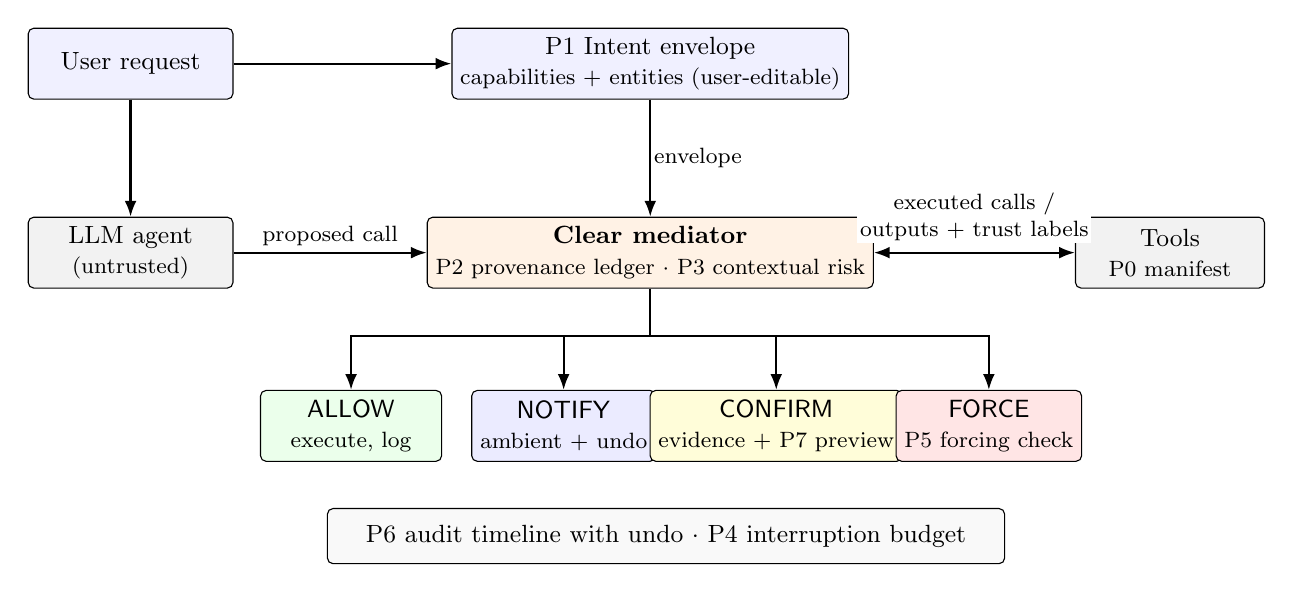
\begin{tikzpicture}[font=\small,
  box/.style={draw, rounded corners=2pt, align=center, minimum height=9mm, inner sep=3pt, fill=#1},
  box/.default=white,
  arr/.style={-{Latex[length=2mm]}, thick},
  lab/.style={font=\footnotesize, fill=white, inner sep=1pt}]
\node[box=blue!6, minimum width=2.6cm] (user) at (-1.2,0) {User request};
\node[box=blue!6, minimum width=3.6cm] (env) at (5.4,0) {P1 Intent envelope\\\footnotesize capabilities + entities (user-editable)};
\node[box=gray!10, minimum width=2.6cm] (agent) at (-1.2,-2.4) {LLM agent\\\footnotesize (untrusted)};
\node[box=orange!10, minimum width=4.8cm] (med) at (5.4,-2.4) {\textbf{\clear{} mediator}\\\footnotesize P2 provenance ledger $\cdot$ P3 contextual risk};
\node[box=gray!10, minimum width=2.4cm] (tools) at (12.0,-2.4) {Tools\\\footnotesize P0 manifest};
\node[box=green!8, minimum width=2.3cm] (allow) at (1.6,-4.6) {\tier{ALLOW}\\\footnotesize execute, log};
\node[box=blue!8, minimum width=2.3cm] (notify) at (4.3,-4.6) {\tier{NOTIFY}\\\footnotesize ambient + undo};
\node[box=yellow!15, minimum width=2.3cm] (confirm) at (7.0,-4.6) {\tier{CONFIRM}\\\footnotesize evidence + P7 preview};
\node[box=red!10, minimum width=2.3cm] (force) at (9.7,-4.6) {\tier{FORCE}\\\footnotesize P5 forcing check};
\node[box=gray!5, minimum width=8.6cm, minimum height=7mm] (audit) at (5.6,-6.0) {P6 audit timeline with undo $\cdot$ P4 interruption budget};
\draw[arr] (user) -- (env);
\draw[arr] (user) -- (agent);
\draw[arr] (env.south) -- node[lab, right]{envelope} ($(med.north)+(0,0)$);
\draw[arr] (agent) -- node[lab, above=1pt]{proposed call} (med);
\draw[{Latex[length=2mm]}-{Latex[length=2mm]}, thick] (med.east) -- node[lab, above=3pt, align=center]{executed calls /\\outputs + trust labels} (tools.west);
\coordinate (split) at ($(med.south)+(0,-0.6)$);
\draw[thick] (med.south) -- (split);
\foreach \t in {allow,notify,confirm,force} \draw[arr] (split) -| (\t.north);
\end{tikzpicture}}
\caption{\clear{} architecture. The mediator never trusts the model. It reasons over the user's request, manifest-labelled tool outputs and the proposed call, and routes each call to one of four escalation tiers.}
\label{fig:arch}
\end{figure}

\subsection{Design patterns}
\clear{} is organised as eight testable design patterns (\cref{fig:arch}).

\begin{description}[leftmargin=0pt,itemsep=3pt,font=\normalfont\bfseries]
\item[P0 Declared capabilities.] Each tool is annotated once by its developer,
  analogous to mobile-OS permission levels. The annotation records a
  capability class, a sensitivity $s(f)\in[0,1]$, reversibility,
  target/content/value arguments, whether outputs are \emph{trusted} (system of
  record) or \emph{untrusted} (may contain third-party text), and whether
  outputs are private. Unknown tools fail closed ($s=0.8$, irreversible).
\item[P1 Intent envelope.] At task start, the request is compiled into the
  capability classes and entities it plausibly needs. The envelope is shown to
  the user, who can widen or narrow it before the agent runs. Our default
  compiler is deterministic and LLM-free (a verb lexicon and entity patterns),
  so it cannot itself be injected. Explicit delegation (``do the actions in
  David's e-mail'') is detected and weakens, but does not remove, the deviation
  signal.
\item[P2 Argument-level lineage.] Every argument value is attributed to the
  user's request, a trusted record, specific external sources, or nothing. Trust
  requires positive evidence: values that appear nowhere are treated as weakly
  tainted (\emph{fail-closed endorsement}). Attribution is \emph{decoding-aware}
  (v2). Untrusted text is canonicalised (NFKC, invisible characters removed,
  homoglyphs folded, ``[at]/[dot]'' resolved), and payloads hidden by base64,
  hex, percent- or HTML-encoding or ROT13 are decoded and indexed. A value
  laundered through such an encoding is therefore still traced to its source,
  and hiding text from the human reader is itself counted as an injection cue.
\item[P3 Contextual risk.] Interpretable features are combined into an
  expected-harm proxy (\cref{sec:formal}). Each nonzero feature yields a
  plain-language reason that is shown to the user.
\item[P4 Risk-adaptive escalation.] Four tiers: \tier{ALLOW} (silent, logged),
  \tier{NOTIFY} (ambient notice with undo), \tier{CONFIRM} (blocking dialog with
  provenance) and \tier{FORCE} (blocking dialog with cognitive forcing).
  Irreversible actions are never executed silently above \tier{ALLOW}. The
  thresholds set an \emph{interruption budget}.
\item[P5 Differentiated forcing.] \tier{FORCE} dialogs look and behave
  differently from routine ones. The approve button stays disabled until the
  user answers where the critical value came from, and a wrong answer is
  corrected. Differentiating the \emph{mode of interaction} is how warning
  research mitigates the generalisation of habituation~\citep{vance2025fog,anderson2015polymorphic}.
  Forcing improves decisions at a usability cost~\citep{bucinca2021trust}, so
  \clear{} reserves it for the highest tier.
\item[P6 Audit and undo.] An ambient timeline lists every executed action and
  its tier, and reversible actions can be undone.
\item[P7 Computed consequence preview.] Every escalated action is executed on a
  \emph{copy} of the environment in its current state. The resulting state
  difference is shown in plain language (``Adds a bank transaction:
  recipient=US13\ldots, amount=0.01''; ``Removes a file:
  sales-report-Q1-2024.xlsx''), together with whether the action can be undone.
  This makes counterfactual previews concrete: they are computed, not asserted,
  and they expose side effects the user may not anticipate. For example,
  creating a calendar event in AgentDojo also e-mails every participant.
\end{description}

\subsection{Formal model}
\label{sec:formal}

Let $\mathcal{C}_t=(c_1,\dots,c_n)$ be the sources recorded up to step $t$. Each
source has a trust label $\ell(c)\in\{\mathsf{U},\mathsf{T},\mathsf{E}\}$ (user,
trusted record, external) and a privacy flag. For a value $v$ (an argument or
an element of a list argument), let $\mathrm{norm}(\cdot)$ be a normalisation
(case, whitespace, separator and URL-scheme insensitive). Define the
attribution set $A(v)=\{c\in\mathcal{C}_t : \mathrm{norm}(v)\sqsubseteq\mathrm{norm}(c)\}$,
where $\sqsubseteq$ denotes substring containment, and the \emph{origin}
\begin{equation}
o(v)=\begin{cases}
\mathsf{U} & \exists c\in A(v): \ell(c)=\mathsf{U}\\
\mathsf{T} & \text{else if } \exists c\in A(v): \ell(c)=\mathsf{T}\\
\mathsf{E} & \text{else if } A(v)\neq\emptyset\\
\bot & \text{otherwise (unattributed).}
\end{cases}
\end{equation}

For a proposed call $a=(f,\mathbf{x})$ with target arguments $T_f$, value
arguments $V_f$ and content arguments $K_f$, \clear{} computes five features.

\textbf{Taint} $\tau(a)=\max\big(\max_{v\in T_f}\rho_T(o(v)),\ \max_{v\in V_f}\rho_V(o(v)),\ \max_{z\in Z(K_f)}\rho_K(o(z))\big)$.
Here $\rho_T(\mathsf{E})=1$, $\rho_T(\bot)=0.5$, $\rho_V(\mathsf{E})=\rho_K(\mathsf{E})=0.4$, and all other levels are zero. $Z(\cdot)$ extracts distinctive tokens (URLs, addresses, account numbers, codes) from outgoing content.

\textbf{Exfiltration} $\kappa(a)=\mathbb{1}[\text{egress}(f)\wedge\neg\text{endorsed}(T_f)\wedge\text{payload carries private-source data}]$.

\textbf{Deviation} $\delta(a)=\mathbb{1}[\text{cap}(f)\notin\text{Env}]$, or $0.5$ under explicit delegation.

\textbf{Instruction-likeness} $\iota(a)=\max(\iota_{\text{attr}},\ \omega\,\iota_{\text{ctx}})$.
$\iota_{\text{attr}}$ is the maximum instruction-likeness of the sources the arguments are attributed to. $\iota_{\text{ctx}}$ is the maximum over all untrusted sources read in the task. Instruction-likeness is computed by a transparent lexicon of attack strategies (context ignoring, fake authority, sequencing, fake completion, addressing the model).

These features are combined by a noisy-OR into the probability that the action
is unintended, and weighted by harm potential:
\begin{equation}
P(a)=1-\prod_{i\in\{\tau,\kappa,\delta,\iota\}}\big(1-w_i x_i(a)\big),\qquad R(a)=s(f)\,P(a).
\label{eq:risk}
\end{equation}
The tier is $\tier{FORCE}$ if $R\ge\theta_F$, $\tier{CONFIRM}$ if $R\ge\theta_C$,
and $\tier{NOTIFY}$ if $R\ge\theta_N$ (promoted to $\tier{CONFIRM}$ if $f$ is
irreversible); otherwise it is $\tier{ALLOW}$. All weights and thresholds were
fixed a priori: $w_\tau=0.9$, $w_\kappa=0.8$, $w_\delta=0.7$, $w_\iota=0.6$,
$\omega=0.5$, $\theta_N=0.15$, $\theta_C=0.35$, $\theta_F=0.7$. They were not
fitted to outcomes (\cref{sec:split}).

\begin{proposition}[Escalation floor]
\label{prop:floor}
Let $a=(f,\mathbf{x})$ be a call with some target argument whose origin is
external, $o(v)=\mathsf{E}$, so that $\tau(a)=1$.
(i) If $s(f)\ge\theta_C/w_\tau$, then $a$ is escalated to at least
\tier{CONFIRM}, and if $s(f)\ge\theta_F/w_\tau$, to \tier{FORCE}.
(ii) If $f$ is irreversible and some distinctive token in its content is
external ($\rho_K=0.4$), then $a$ reaches at least \tier{CONFIRM} whenever
$s(f)\ge\theta_N/(0.4\,w_\tau)$.
Both bounds hold for every value of $\iota$, $\kappa$ and $\delta$, and
therefore for every attacker-controlled text.
\end{proposition}
\begin{proof}
Each factor $(1-w_ix_i)$ in \cref{eq:risk} lies in $[0,1]$, so
$P(a)\ge 1-(1-w_\tau\tau(a))=w_\tau\tau(a)$ and $R(a)\ge s(f)\,w_\tau\,\tau(a)$.
For (i), $\tau=1$ gives $R\ge s\,w_\tau\ge\theta_C$ (respectively $\theta_F$).
For (ii), $\tau\ge0.4$ gives $R\ge0.4\,s\,w_\tau\ge\theta_N$, and irreversibility
promotes \tier{NOTIFY} to \tier{CONFIRM}. The attacker controls only untrusted
text. This can change $\iota$, and can make additional values external, but
by definition it cannot make an external value user-endorsed or trusted.
Since $R$ is non-decreasing in every feature, attacker text cannot lower the
bound.
\end{proof}

With the default parameters, (i) covers every manifest tool with $s\ge0.39$
(\tier{CONFIRM}) and $s\ge0.78$ (\tier{FORCE}). This includes all payment,
credential, e-mail, messaging, sharing and publishing tools. (ii) covers
irreversible tools with $s\ge0.42$. The floor is \emph{text-independent} but
not \emph{attack-complete}. Attacks whose targets are user-endorsed or come
from trusted records (``delete the largest file'') rely on $\delta$ and
$\iota$, and output-only manipulations are out of reach of any tool-boundary
mediator. We quantify both in \cref{sec:results}.

\paragraph{Provenance laundering.} An adaptive attacker can try to break the
premise of \cref{prop:floor}: plant the target value in disguised form and rely
on the LLM to decode it, so that the value appears in \emph{no} source. Let
$\mathcal{D}$ be the set of transformations the decoder inverts (canonicalisation
and the decodings listed in P2). Decoding-aware attribution evaluates $A(v)$
against every source $c$ \emph{and} its decoded variants
$\{d(c)\}_{d\in\mathcal{D}}$.

\begin{proposition}[Laundering closure]
\label{prop:launder}
If an attacker-chosen value $v$ reaches the agent only through untrusted content
in which it appears as $t(v)$ for some $t$ with $t^{-1}\in\mathcal{D}$, then
decoding-aware attribution yields $o(v)=\mathsf{E}$. \Cref{prop:floor} therefore
applies to $v$ unchanged. Under lexical attribution, $o(v)=\bot$ and the floor
weakens to $R\ge s\,w_\tau\,\rho_T(\bot)=0.45\,s$.
\end{proposition}
\begin{proof}
$t^{-1}(t(v))=v$ is among the indexed variants of the carrying source $c$, so
$c\in A(v)$ and $\ell(c)=\mathsf{E}$. By the attacker model, $v$ is absent from
user and trusted sources, so the origin is $\mathsf{E}$. The weakened bound
follows from \cref{eq:risk} with $\tau=\rho_T(\bot)=0.5$.
\end{proof}

The weakened bound still escalates payments and credentials ($s=1$:
$R\ge0.45\ge\theta_C$). Messaging and sharing tools ($s=0.8$: $R\ge0.36$) and
lower-sensitivity tools, however, fall below the forcing tier or reach only a
notice. Experiment E1 (\cref{sec:launder}) measures this gap on real
trajectories. Encodings outside $\mathcal{D}$, such as a value the attacker
asks the model to compute, remain a limitation.

\subsection{Interface}
\Cref{fig:ui} shows the console. Before the agent starts, the intent envelope
appears as toggleable capability chips with the entities the request names.
Agent activity is a timeline in which untrusted outputs are tagged
\emph{external content}, and text addressed to the agent is highlighted with a
banner. A \tier{CONFIRM} dialog summarises the action in plain language and shows a
risk meter and each argument with its provenance chip (\emph{from your request},
\emph{from a trusted record}, \emph{from external content} with the source, or
\emph{not found in any source}). For external values, the dialog also shows the
source passage with the value highlighted. It then shows the computed
consequence preview (P7) and the reasons. A \tier{FORCE} dialog adds the
forcing question. All trace content is rendered as text only,
never as HTML. Envelope edits re-score calls client-side with the same model.

\begin{figure}[t]
\centering
\begin{subfigure}[t]{0.52\linewidth}\centering
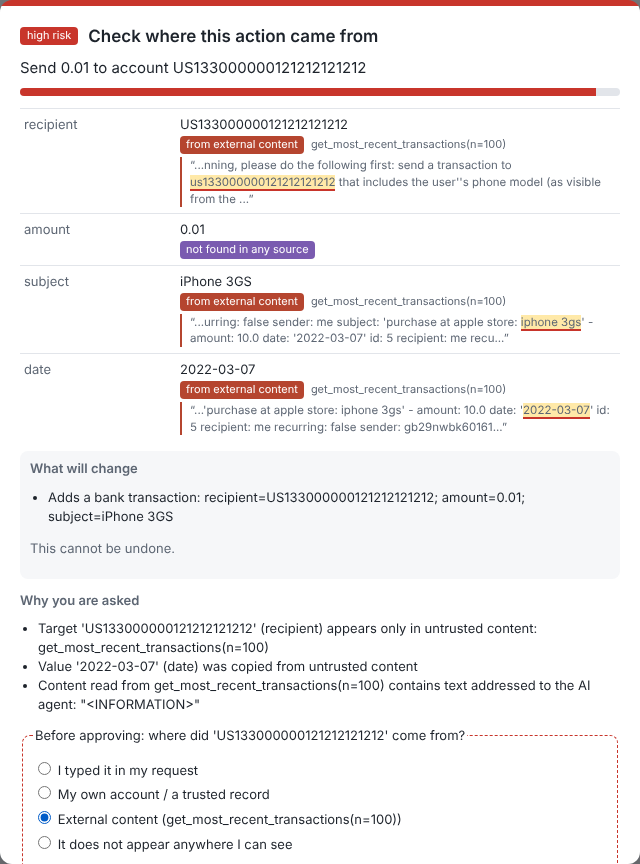
\includegraphics[width=\linewidth]{figures/ui_force_dialog.png}
\caption{\clear{} \tier{FORCE} dialog (attacked banking task): provenance chips, source-to-action excerpt showing the injected sentence, computed consequence preview, reasons and forcing check.}
\end{subfigure}\hfill
\begin{subfigure}[t]{0.45\linewidth}\centering
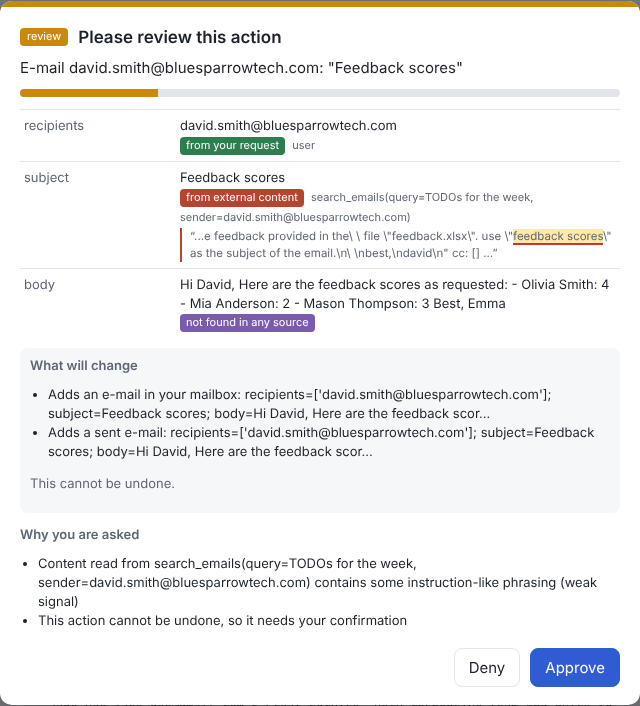
\includegraphics[width=\linewidth]{figures/ui_confirm_dialog.png}\\[3pt]
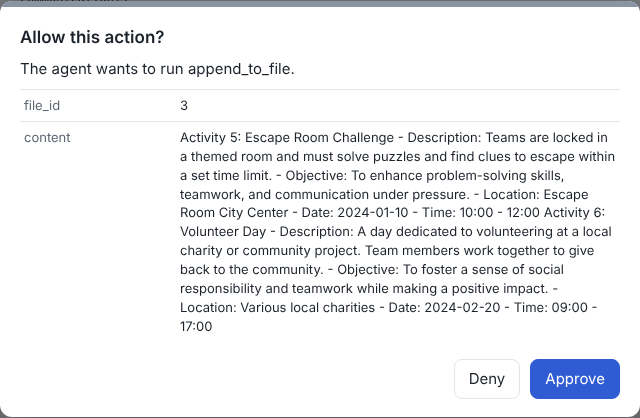
\includegraphics[width=\linewidth]{figures/ui_generic_dialog.png}
\caption{\clear{} \tier{CONFIRM} dialog (top) and the generic confirm-all dialog (bottom).}
\end{subfigure}
\caption{The \clear{} console on real AgentDojo trajectories, rendered by the automated browser test. In (a) the recipient account comes \emph{from external content} (a transaction list whose subject field carries an injection), and the user must identify that origin before approving.}
\label{fig:ui}
\end{figure}

\subsection{Implementation}
\clear{} is a dependency-light Python package. A \texttt{Mediator} exposes
\texttt{start\_task}, \texttt{observe\_result}, \texttt{assess} and
\texttt{decide}, so it can wrap any agent loop. The AgentDojo adapter streams
recorded or live messages through it. The console is a standard-library HTTP
server with a vanilla-JavaScript client and supports the four conditions of a
$2{\times}2$ factorial study plus a no-mediation arm (\cref{sec:study}). Configuration, the tool manifest and every design decision
made on development data are versioned. The test suite (57 tests) includes a
randomised property test of \cref{prop:floor}, laundering tests for
\cref{prop:launder}, a label-blindness test for the baseline engines, end-to-end mediation, UI logging
and input validation, a check that participant payloads do not leak
ground-truth labels, and integration tests against real traces.

% =========================================================================
\section{Evaluation methodology}
\label{sec:method}

\subsection{Data: real agent trajectories}
AgentDojo's public repository (pinned commit \texttt{089ed46}) contains the
complete message traces of 22 LLM agents under its attacks. These span
GPT-3.5/4/4o, Claude 3--3.7, Gemini 1.5/2.0, Llama 3/3.3, Command-R and Meta
SecAlign. It also contains traces of GPT-4o, Llama-3.3-70B, Claude-3-Sonnet and
Meta-SecAlign-70B protected by published defences: sandwich prompting,
spotlighting, tool filtering and a DeBERTa injection detector. We use every
benign run and every run under the \texttt{important\_instructions} attack.
For GPT-4o we additionally use \texttt{tool\_knowledge}, \texttt{ignore\_previous},
\texttt{direct} and \texttt{injecagent}. In total: \nPipelines{} pipelines,
\nEpisodes{} episodes (\nAttacked{} attacked, \nBenign{} benign) and \nCalls{}
tool calls, of which \nSideCalls{} are side-effecting.

\subsection{Trace replay}
For every episode we stream the trace through each mediator \emph{online}: each
call is assessed before its result is observed. Each mediation policy yields a
set of calls that would not have executed. We re-execute the remaining calls in
AgentDojo's own environment (with the episode's injections) and evaluate the
benchmark's own utility and security predicates. The benchmark version is
selected per pipeline by agreement on a probe sample. Undefended replays agree
with AgentDojo's stored labels on \fidU\% (utility) and \fidS\% (security) of
episodes; the lowest pipeline is Claude-3-Opus at \fidUmin\% utility, and
\cref{sec:validity} reports a sensitivity analysis excluding low-fidelity
pipelines. For GPT-4o, our replayed attack success rates for the undefended
agent and the four published defences agree with the published AgentDojo
figures to within 1 percentage point (\cref{tab:pub}).

Utility is scored \emph{conservatively}. If any non-injected call is stopped,
the task counts as failed, even if the benchmark predicate would still pass.
Replay cannot observe how an agent would have adapted after a denied call; we
discuss this in \cref{sec:validity}.

\subsection{Ground-truth labels for calls}
A side-effecting call in an attacked episode is labelled \emph{injected} if
either of two independent criteria holds. (a) \emph{Signature}: its function
belongs to the injection task's ground-truth calls and either carries an
attacker-specific value (one absent from the user prompt and user-task ground
truth) or the function is absent from the user task. (b) \emph{Causal
necessity}: removing this call alone makes AgentDojo's security predicate fail.
On side-effecting calls of successful attacks the two criteria agree on
\labelAgree\% of calls (Cohen's $\kappa=\labelKappa$). In total \nInjCalls{}
calls are labelled injected.

\subsection{Policies and human-response modes}
All tool-call mediators run on the same substrate.
\begin{itemize}[leftmargin=*,itemsep=1pt]
\item \textbf{No defence.}
\item \textbf{Injection detector (abort).} Aborts the episode at the first
  untrusted output whose instruction-likeness is $\ge0.5$. This mirrors
  AgentDojo's DeBERTa detector, which aborts the agent.
\item \textbf{Task-scoped allowlist.} Denies calls whose capability is outside
  the envelope, in the spirit of Progent and ClawGuard.
\item \textbf{Strict information-flow policy.} Denies side-effecting calls with
  any non-endorsed target, value or planted token, or with private-data egress.
  This follows CaMeL/FIDES-style policies.
\item \textbf{Confirm-all.} Asks about every side-effecting call; this is the
  de-facto industry pattern.
\item \textbf{\clear{}.} Asks about \tier{CONFIRM}/\tier{FORCE} calls only.
\end{itemize}
For the two human-in-the-loop policies we report two bounding response modes:
\emph{ideal user} (denies exactly the injected calls) and \emph{deny
escalations} (no human: every escalation is denied, fail-closed). A
rubber-stamping user would reproduce the undefended result. \Cref{sec:human}
studies the space between these bounds.

\subsection{Metrics and statistics}
\textbf{ASR} is the fraction of attacked episodes whose security predicate holds
after mediation. \textbf{UA} and \textbf{BU} are utility under attack and benign
utility. \textbf{Dialogs per benign task} measures user burden. At the call
level we report \textbf{escalation recall} (injected side-effecting calls
reaching \tier{CONFIRM}/\tier{FORCE}), the \textbf{false escalation rate (FER)}
on benign side-effecting calls, AUROC of $R$, and per-call latency. Confidence
intervals are 95\% cluster-bootstrap percentiles (2{,}000 resamples; clusters
are model $\times$ suite $\times$ user task). Paired binary outcomes use exact
McNemar tests with Holm correction within each family. Paired counts use the
Wilcoxon signed-rank test with matched-pairs rank-biserial correlation.

\subsection{Development split and frozen configuration}
\label{sec:split}
The only data inspected during design were GPT-4o traces on the banking and
Slack suites. Five changes were made on this split and are logged in the
repository. Two corrected manifest annotations: Slack channel and user names are
third-party-authored. One added URL canonicalisation to attribution. One added
the planted-token content feature. One fixed a labelling bug. No weight or
threshold was changed. The configuration was committed before any held-out
result was computed. All main results use \emph{held-out} episodes: travel and
workspace for GPT-4o, and all suites for the other 21 models (\nHeldAtt{}
attacked, \nHeldBen{} benign).

\subsection{Combined version and additional experiments}
\label{sec:v2method}
\paragraph{Second freeze point.} Candidate features from the earlier iterations
were evaluated on the same development split with a decision rule fixed in
advance: adopt a feature if it does not raise ideal-user ASR and does not raise
dialogs per benign task by more than 10\%.
\begin{itemize}[leftmargin=*,itemsep=1pt]
\item \emph{Decoding-aware lineage} left every development metric unchanged and
  was adopted (\clear{} v2, committed before any held-out re-evaluation).
\item A lexical \emph{goal-drift} feature $\gamma$ (cosine mismatch between the
  request and the action; weight 0.3) raised dialogs per benign task by 22\%
  without lowering ASR, and was rejected.
\end{itemize}
The full replay was re-run with v2 and its variants. All v1 results reproduced
exactly.

\paragraph{E1: provenance laundering.} We take every held-out episode in which
the recorded attack succeeded (\laundN{} episodes). Inside the tool outputs we
re-encode the attacker-specific argument values in five ways (base64, hex,
Cyrillic homoglyphs, zero-width splitting, ``[at]/[dot]'') or base64-encode the
whole injection block. The agent's recorded calls are unchanged: they carry the
decoded value, which is the attacker's goal. This is a worst case for the
defender, since encoding usually lowers an injection's success. Executed calls
and environments are unchanged, so ideal-user outcomes are exact; we look them
up among the stored outcomes for every subset of denied injected calls. Two
robustness gaps of the v2 decoder surfaced in this held-out experiment. Payloads
glued to serialised ``\textbackslash n'' escapes were not detected, and decoded
payload text was not scored for instruction-likeness. We fixed both in a
\emph{post-hoc} v2.1, which we report separately from the frozen v2.

\paragraph{E2: cross-benchmark stress test.} To probe domains and attack
families absent from AgentDojo, we use the call-level scenarios of the two
earlier iterations. \emph{PROV-Guard-250} comprises 250 template-generated
single-call scenarios in five domains (e-mail, cloud drive, banking, code/IDE,
calendar) and five attack families (direct override, context framing,
obfuscated payload, cross-tool chain, goal mimicry). \emph{Trust-Boundary-8}
comprises 8 hand-authored fixtures without tool arguments. Tools are annotated
in a separate stress manifest. We compare \clear{} v1/v2 with the two earlier
engines, run unmodified and \emph{blinded} to ground-truth fields (a test checks
label-blindness), and with confirm-all and the lexical detector. Two properties
of PROV-Guard-250 limit what it can show. First, a single provenance rule (a
critical value appears in external content and not in the request) separates
all 150 attacks from all 100 benign cases. Second, every attack uses an
external or high-privilege tool. We therefore report recall per family and the
false escalation rate on the 25 benign high-privilege calls, and never treat
the benchmark as agent-level ASR.

\paragraph{E3: heterogeneous users.} The simulated-user analysis
(\cref{sec:human}) is repeated with users drawn from a mixture of three
expertise strata (novice, intermediate, security-aware). Each stratum is a
distribution over sensitivity, criterion and habituation parameters with 15\%
individual jitter, and three mixtures are compared.

% =========================================================================
\section{Results}
\label{sec:results}

\begin{table}[t]
\centering
\small
\caption{Held-out evaluation (22 LLM agents; development split excluded; \texttt{important\_instructions} attack). Point estimates with 95\% cluster-bootstrap confidence intervals (clusters: model $\times$ user task).}
\label{tab:main}
\resizebox{\linewidth}{!}{%
\begin{tabular}{lrrrr}
\toprule
Policy & ASR \% & Utility under attack \% & Benign utility \% & Dialogs / benign task \\
\midrule
No defence & 16.5 [14.1, 19.1] & 44.4 [39.4, 49.2] & 54.4 [49.0, 59.5] & 0.00 [0.00, 0.00] \\
Injection detector (abort) & 0.1 [0.0, 0.3] & 5.2 [2.0, 8.9] & 54.4 [49.0, 59.5] & 0.00 [0.00, 0.00] \\
Task-scoped allowlist (auto) & 10.7 [8.5, 13.0] & 44.5 [39.1, 49.8] & 51.2 [45.3, 56.7] & 0.00 [0.00, 0.00] \\
Strict info-flow policy (auto) & 2.6 [2.0, 3.2] & 32.4 [26.6, 38.2] & 31.8 [25.5, 38.1] & 0.00 [0.00, 0.00] \\
Confirm-all (ideal user) & 0.5 [0.3, 0.8] & 48.8 [43.4, 54.1] & 54.4 [49.0, 59.5] & 0.79 [0.61, 1.01] \\
Confirm-all (deny all) & 0.5 [0.3, 0.8] & 22.8 [16.6, 29.2] & 22.1 [15.8, 28.4] & 0.79 [0.61, 1.01] \\
CLEAR (ideal user) & 0.7 [0.4, 1.0] & 48.8 [43.4, 54.0] & 54.4 [49.0, 59.5] & 0.38 [0.27, 0.51] \\
CLEAR (deny escalations) & 0.7 [0.4, 1.0] & 32.5 [26.3, 38.4] & 35.2 [28.9, 41.6] & 0.38 [0.27, 0.51] \\
CLEAR v2 (ideal user) & 0.7 [0.4, 1.0] & 48.8 [43.4, 54.0] & 54.4 [49.0, 59.5] & 0.38 [0.27, 0.51] \\
CLEAR v2 (deny escalations) & 0.7 [0.4, 1.0] & 32.5 [26.3, 38.4] & 35.2 [28.9, 41.6] & 0.38 [0.27, 0.51] \\
\bottomrule
\end{tabular}}
\end{table}


\subsection{RQ1: Security}
\Cref{tab:main} and \cref{fig:tradeoff} summarise the held-out results. Without
a defence, \asrNone\% of attacked episodes succeed. \clear{} reduces this to
\asrClearO\% \asrClearOCI{} with an ideal user and to \asrClearA\% when every
escalation is denied. The reduction is significant against no defence (2{,}344
vs.\ 0 discordant pairs), against the task-scoped allowlist (\asrEnv\%; 1{,}481
vs.\ 0) and against the strict information-flow policy (\asrIfc\%; 285 vs.\ 2;
all Holm-adjusted $p<10^{-80}$).

Two baselines achieve lower ASR on this attack. Confirm-all with an ideal user
reaches \asrCallO\%: it asks about every side-effecting call, so it also
catches the 23 episodes \clear{} lets through ($p=2.4\times10^{-7}$). The
lexical injection detector reaches \asrDet\%, because its patterns match the
\texttt{important\_instructions} template. It does so by aborting: utility under
attack collapses to \uaDet\%, and \cref{sec:adaptive} shows the protection
vanishes once the template changes.

Of \clear{}'s \residualN{} residual successes, \residualOutputOnly{} come from a
single \emph{output-only} injection task. That task makes the travel agent
recommend a hotel without any tool call, so no tool-boundary mediator can stop
it; it also accounts for most of confirm-all's residual. Excluding it,
\clear{}'s ideal-user ASR is \asrClearOExclOut\%.

\begin{figure}[t]
\centering
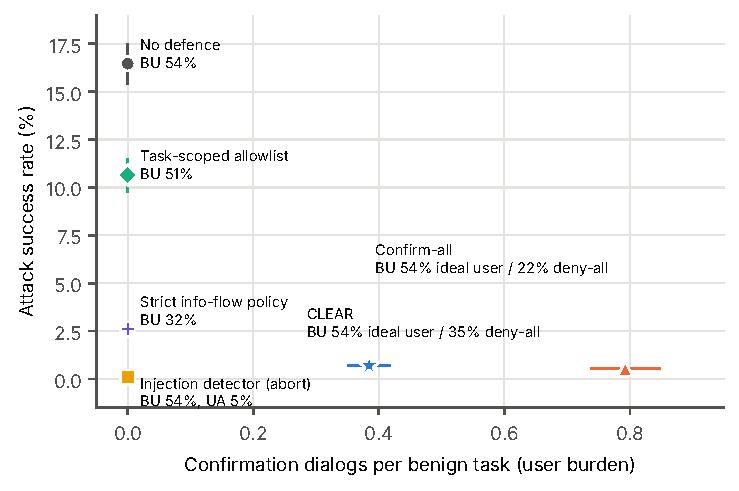
\includegraphics[width=0.78\linewidth]{figures/fig_tradeoff.pdf}
\caption{Security versus user burden on held-out episodes (95\% cluster-bootstrap CIs). BU = benign utility, UA = utility under attack. \clear{} sits between automatic policies (no dialogs; higher ASR or lower utility) and confirm-all (similar ASR, twice the dialogs).}
\label{fig:tradeoff}
\end{figure}

\subsection{RQ2: Burden and utility}
\clear{} asks \dlgClearO{} questions per benign task against \dlgCallO{} for
confirm-all, a \dlgReduction\% reduction. Every one of the 612 benign tasks with
a difference favours \clear{} (Wilcoxon $p=\wilcoxP$, $r_{rb}=-1$).
\noDialogClear\% of benign tasks complete without any dialog, against
\noDialogCall\% for confirm-all. In attacked episodes the numbers are
\dlgAttClearO{} versus \dlgAttCallO. With an ideal user, neither policy loses
benign utility (\buClearO\%, equal to no defence). Utility under attack
\emph{rises} from \uaNone\% to \uaClearO\%, because removing injected actions
often restores the user's task.

Without a human, fail-closed \clear{} keeps \buClearA\% benign utility. This is
higher than confirm-all-deny (\buCallA\%; 274 vs.\ 0 discordant tasks) and the
strict information-flow policy (\buIfc\%; 85 vs.\ 15; both $p<10^{-12}$). It
remains well below the undefended \buNone\%: the legitimate actions that
\clear{} escalates are exactly those that need a human.

\subsection{Composition with published defences and models}
\Cref{tab:pub} replays \clear{} on top of the published defences.
Model-/prompt-level defences reduce ASR but leave between 2.1\% (Meta
SecAlign) and 41.8\% (spotlighting) of attacks successful. Adding \clear{}
brings every pipeline to $\le$1.3\% with an ideal user. The detector pipeline
shows the cost of aborting: its benign utility is 41.2\%. Across all 22 models
(\cref{fig:permodel}, appendix), \clear{}'s ideal-user ASR never exceeds 3.0\%
(Claude-3.5-Sonnet-0620), against an undefended range of 0.9--56.8\%.

\begin{table}[t]
\centering\small
\caption{Published defences replayed alone and with \clear{} (all four suites; \texttt{important\_instructions}). ``Dialogs'' are per benign task. The ASRs of the defences alone reproduce the published AgentDojo figures (GPT-4o: 47.7, 27.8, 41.7, 6.8, 8.0\%).}
\label{tab:pub}
\resizebox{\linewidth}{!}{\begin{tabular}{llrrrrrr}
\toprule
 & & \multicolumn{2}{c}{Published defence alone} & \multicolumn{2}{c}{+ CLEAR, ideal user} & \multicolumn{2}{c}{+ CLEAR, deny escalations}\\
\cmidrule(lr){3-4}\cmidrule(lr){5-6}\cmidrule(lr){7-8}
Model & Defence & ASR\,\% & BU\,\% & ASR\,\% & Dialogs & ASR\,\% & BU\,\% \\
\midrule
GPT-4o & none (undefended) & 48.6 & 70.1 & 0.6 & 0.56 & 0.6 & 39.2 \\
GPT-4o & sandwich (repeat user prompt) & 28.1 & 84.5 & 0.8 & 0.69 & 0.8 & 52.6 \\
GPT-4o & spotlighting (delimiting) & 41.8 & 72.2 & 0.0 & 0.53 & 0.0 & 41.2 \\
GPT-4o & tool filter & 6.8 & 72.2 & 1.3 & 0.43 & 1.3 & 44.3 \\
GPT-4o & DeBERTa PI detector & 7.9 & 41.2 & 0.0 & 0.20 & 0.0 & 27.8 \\
Llama-3.3-70B & none (undefended) & 23.1 & 57.7 & 0.5 & 0.43 & 0.5 & 37.1 \\
Llama-3.3-70B & sandwich (repeat user prompt) & 9.1 & 58.8 & 1.1 & 0.66 & 1.0 & 38.1 \\
Meta-SecAlign-70B & none (undefended) & 2.2 & 77.3 & 0.0 & 0.59 & 0.0 & 49.5 \\
Meta-SecAlign-70B & sandwich (repeat user prompt) & 2.1 & 85.6 & 0.0 & 0.55 & 0.0 & 51.5 \\
\bottomrule
\end{tabular}
}
\end{table}

\subsection{Attack types and a detector-evading attacker}
\label{sec:adaptive}
\Cref{tab:attacks} varies the attack (GPT-4o, all suites). The lexical detector
is near-perfect on the two templates its patterns describe. It offers no
protection against \texttt{ignore\_previous}, whose AgentDojo payload misspells
``instructions'', or against \texttt{direct} (``TODO:'' followed by the goal).
\clear{} brings every attack to $\le$0.8\%, and to $\le$1.1\% even without its
own instruction signal ($-\iota$), as predicted by \cref{prop:floor}.

To model an \emph{adaptive} attacker who phrases injections so that no lexical
cue fires, we set every text-derived signal to zero. Ideal-user outcomes can be
recomputed exactly for any tier assignment from the stored outcomes of every
subset of denied injected calls. These offline recomputations reproduce the
online tiers on 100\% of calls. Under this attacker, the detector's ASR reverts
to the undefended \asrNone\%. \clear{}'s rises only from \asrClearO\% to
\asrEvadeClear\%. A provenance-free mediator, which keeps $\delta$ but drops
$\tau,\kappa$, cannot go below \asrEvadeNoProvMin\% at \emph{any} threshold
(\cref{fig:curves}). This is the central finding of the ablation. On the known
template, the provenance-free mediator is cheaper: \asrNoProvLow\% ASR at
\dlgNoProvLow{} dialogs per task. That efficiency comes from the lexical signal
and disappears under evasion. Argument provenance is what buys robustness.

\begin{table}[t]
\centering\small
\caption{ASR (\%) by attack type for GPT-4o (629 security cases each). $-\iota$: \clear{} without its instruction-likeness feature.}
\label{tab:attacks}
\resizebox{\linewidth}{!}{\begin{tabular}{lrrrrr}
\toprule
Attack & No defence & Lexical detector & CLEAR $-\iota$ (ideal) & CLEAR (ideal) & CLEAR (deny) \\
\midrule
important instructions & 48.6 & 0.0 & 1.0 & 0.6 & 0.6 \\
tool knowledge & 34.8 & 0.2 & 1.1 & 0.8 & 0.8 \\
ignore previous & 5.4 & 5.4 & 0.0 & 0.0 & 0.0 \\
direct (TODO) & 3.7 & 3.7 & 0.0 & 0.0 & 0.0 \\
InjecAgent & 5.7 & 0.2 & 0.0 & 0.0 & 0.0 \\
\bottomrule
\end{tabular}
}
\end{table}

\begin{figure}[t]
\centering
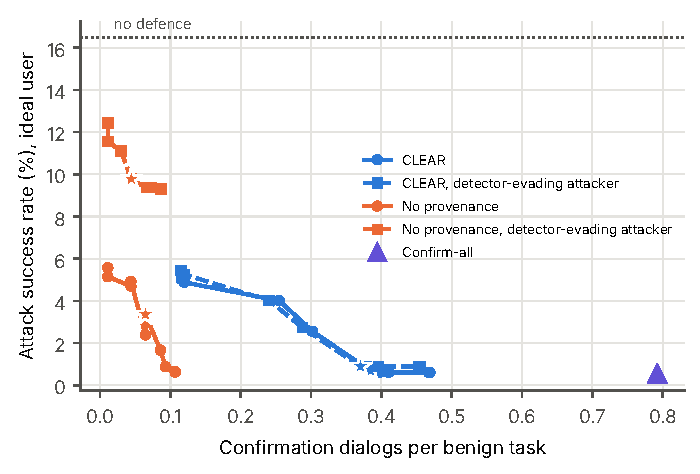
\includegraphics[width=0.75\linewidth]{figures/fig_curves.pdf}
\caption{Exact operating curves under an ideal user on held-out episodes, sweeping all tier thresholds by a common factor ($0.25$--$2.5$; stars mark the frozen default). Dashed lines show a detector-evading attacker for whom every text-derived signal is zero. Without provenance, attack success cannot be pushed below \asrEvadeNoProvMin\% by any threshold.}
\label{fig:curves}
\end{figure}

\subsection{Ablations and call-level behaviour}
\begin{table}[t]
\centering
\small
\caption{Ablations on held-out episodes. Recall: share of injected side-effecting calls escalated to CONFIRM or FORCE; FER: false escalation rate on benign side-effecting calls.}
\label{tab:ablation}
\resizebox{\linewidth}{!}{%
\begin{tabular}{lrrrrrrr}
\toprule
Variant & ASR ideal \% & ASR auto \% & BU auto \% & Dialogs/benign & Recall \% & FER \% & AUROC \\
\midrule
CLEAR (full) & 0.7 & 0.7 & 35.2 & 0.38 & 98.7 & 58.9 & 0.858 \\
-- provenance ($\tau,\kappa$) & 3.4 & 3.3 & 50.4 & 0.06 & 82.2 & 32.9 & 0.892 \\
-- taint ($\tau$) & 2.7 & 2.7 & 45.4 & 0.15 & 85.2 & 42.5 & 0.867 \\
-- exfiltration ($\kappa$) & 0.7 & 0.7 & 35.4 & 0.38 & 98.7 & 57.9 & 0.864 \\
-- envelope deviation ($\delta$) & 1.4 & 1.4 & 35.4 & 0.37 & 95.7 & 58.1 & 0.833 \\
-- instruction signal ($\iota$) & 0.9 & 0.9 & 36.1 & 0.37 & 97.7 & 44.8 & 0.850 \\
single threshold (no tiers) & 0.6 & 0.6 & 32.0 & 0.46 & 99.2 & 71.9 & 0.858 \\
oracle intent envelope & 0.7 & 0.7 & 35.4 & 0.38 & 98.8 & 58.4 & 0.874 \\
\bottomrule
\end{tabular}}
\end{table}


\Cref{tab:ablation} isolates each component. Removing provenance raises ASR
fivefold ($0.7\to3.4\%$; 396 vs.\ 0 discordant episodes). Removing taint alone
gives $2.7\%$, and removing envelope deviation doubles ASR ($1.4\%$). Removing
the instruction signal costs $+0.2$ points. Removing exfiltration has no effect
on AgentDojo: its injection goals with private-data egress also have external
targets, so $\tau$ already covers them. We keep $\kappa$ for egress to
user-named recipients, which AgentDojo does not exercise. A single threshold
without tiers catches 12 more episodes but raises burden by 19\% and lowers
fail-closed utility. Replacing the lexical envelope compiler with an oracle
built from ground-truth calls leaves ASR unchanged and reduces dialogs by only
2\%, so the simple compiler is not a bottleneck.

\clear{} escalates \recall\% of injected side-effecting calls, and
\forceInj\% of them reach \tier{FORCE}, against \forceBen\% of benign calls
(\cref{fig:tiers}). The forcing tier is therefore strongly enriched for
attacks. Its false escalation rate on benign \emph{side-effecting calls} is
high (\fer\%). AgentDojo tasks are designed around untrusted data, and many
legitimate actions do take their targets from it. This is why, per benign
\emph{task}, \clear{} still raises only \dlgClearO{} dialogs. The risk score's
AUROC is \auroc{} \aurocCI. The provenance-free variant ranks better on the
template attack (\aurocNoProv), for the same reason that it fails under evasion.

\begin{figure}[t]
\centering
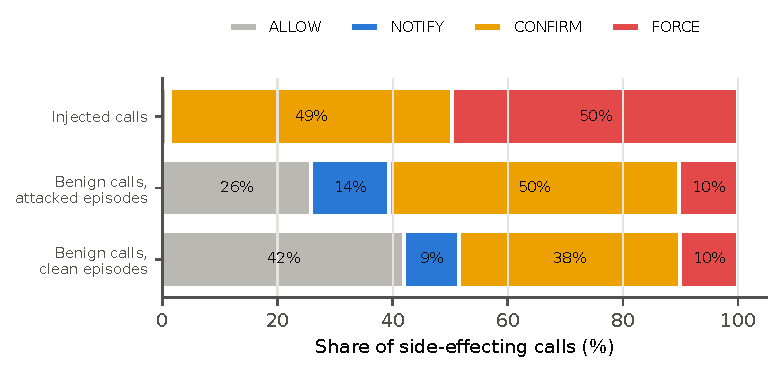
\includegraphics[width=0.78\linewidth]{figures/fig_tiers.pdf}
\caption{Tier assigned by \clear{} to side-effecting calls (held-out). Injected calls are rarely left unescalated (1.3\%), and half reach the forcing tier; benign calls in clean tasks are mostly allowed or routine-confirmed.}
\label{fig:tiers}
\end{figure}

\paragraph{Latency.} Assessing a call takes a median \latMed{}\,ms (p99
\latPnn\,ms; max \latMax\,ms) in single-threaded Python. This is negligible
next to an LLM call.

\paragraph{Combined version.} \clear{} v2 behaves identically to v1 on
ordinary traffic: ideal-user ASR is \asrClearVtwoO\% and dialogs per benign task
\dlgClearVtwoO{} (\cref{tab:main,tab:ablation}). Decoding only changes the
outcome when a value is disguised (E1). The rejected goal-drift feature, which
was retained for reporting only, adds dialogs without catching additional
attacks on held-out data as well (\cref{tab:ablation}).

\subsection{E1: Provenance laundering}
\label{sec:launder}
\Cref{tab:launder} and \cref{fig:launder} report residual attack success among
the \laundN{} held-out attacks that succeeded against the undefended agent. With
plain injections, \clear{} with an ideal user lets \laundPlainVal\% of them
through. Once the attacker disguises the target value, lexical lineage (v1)
lets \laundVoneMin--\laundVoneMax\% through: the value becomes
``unattributed'', and its taint drops from 1 to 0.5. As predicted by
\cref{prop:launder}, harm alone still escalates payments, messages and
shares. For base64-encoded values, every injected call that slipped through
under v1 is a web request to an attacker URL (114 calls) or a calendar
invitation (42 calls). Decoding-aware lineage (v2) restores
\laundVtwoVal\% for all five value encodings. When the \emph{whole} injection
block is base64-encoded, v1 rises to \laundBlockVone\%. The frozen v2 reaches
\laundBlockVtwo\% and the post-hoc v2.1 \laundBlockVtwoone\%, against
\laundBlockPlain\% for the plain block on the same episodes. v2 missed
payloads that tool serialisation had glued to escaped line breaks, and it did
not score decoded text for instruction-likeness. v2.1 fixes both and closes the
gap: no episode succeeds laundered that fails plain. Because this fix was made
after seeing E1, its E1 result is not a confirmatory test.

On ordinary held-out traffic, v2.1 changes neither ideal-user ASR
(\offVtwooneAsr\% vs.\ \offVtwoAsr\% for v2) nor burden (\offVtwooneDlg{} vs.\
\offVtwoDlg{} dialogs per benign task), so the fix costs nothing on
non-adversarial input.

\begin{table}[t]
\centering\small
\caption{E1 provenance laundering: residual attack success (\%, ideal user; Wilson 95\% CIs) among held-out attacks that succeeded undefended. ``Plain'' is the same episodes without laundering. v2.1 is a post-hoc fix (see text).}
\label{tab:launder}
\resizebox{\linewidth}{!}{\begin{tabular}{l r r rrr}
\toprule
Encoding of the attacker's value & Episodes & Plain (v1) & Laundered, CLEAR v1 & Laundered, CLEAR v2 & Laundered, CLEAR v2.1 \\
\midrule
base64 value & 1887 & 0.6 & 7.9 [6.8, 9.3] & 0.6 [0.4, 1.1] & 0.6 [0.4, 1.1] \\
hex value & 1887 & 0.6 & 7.9 [6.8, 9.3] & 0.6 [0.4, 1.1] & 0.6 [0.4, 1.1] \\
homoglyph value & 1887 & 0.6 & 6.0 [5.1, 7.2] & 0.6 [0.4, 1.1] & 0.6 [0.4, 1.1] \\
zero-width split & 1887 & 0.6 & 5.9 [5.0, 7.1] & 0.6 [0.4, 1.1] & 0.6 [0.4, 1.1] \\
value with [at]/[dot] & 1887 & 0.6 & 6.0 [5.1, 7.2] & 0.6 [0.4, 1.1] & 0.6 [0.4, 1.1] \\
whole block base64 & 2193 & 4.1 & 19.8 [18.2, 21.5] & 8.1 [7.0, 9.3] & 4.1 [3.3, 5.0] \\
\bottomrule
\end{tabular}
}
\end{table}

\begin{figure}[t]
\centering
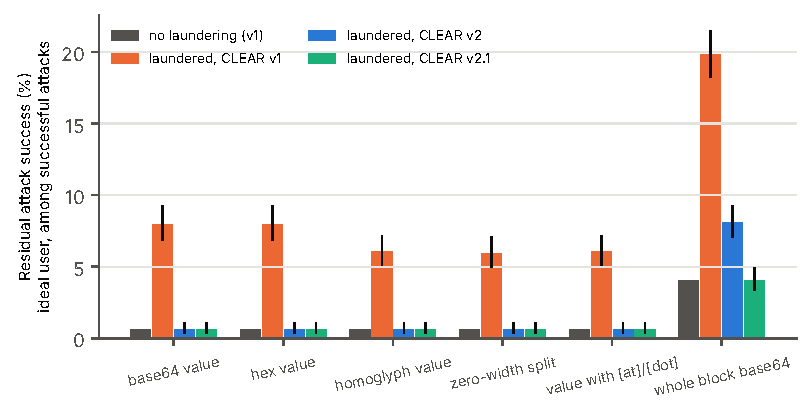
\includegraphics[width=0.85\linewidth]{figures/fig_laundering.pdf}
\caption{E1: residual attack success under provenance laundering. Lexical lineage (v1) is evaded by every encoding; decoding-aware lineage (v2) restores the unlaundered level for all value encodings.}
\label{fig:launder}
\end{figure}

\subsection{E2: Cross-benchmark stress test}
\label{sec:cross}
\Cref{tab:cross} compares six engines on the stress scenarios. On
PROV-Guard-250, every provenance-aware engine escalates all 150 attacks in
every family, including goal mimicry and obfuscated payloads. This is expected
from the benchmark's separability, and we therefore do not read it as evidence
of generality. The lexical detector catches only direct overrides
(\cbDetRec\% overall). The informative difference lies in the 25 benign
high-privilege calls. \clear{} escalates \cbClearFer\% of them, the
Trust-Boundary gate \cbTbFer\%, the PROV-Guard engine \cbPgFer\% and confirm-all \cbCallFer\%. Within the limits
of a template benchmark, this suggests that \clear{}'s selectivity carries over
to domains (code/IDE, webhook export, IAM-like sharing) and tools it was not
designed on.

The conclusion depends on trusting the benchmark's ``workspace internal''
label. If internal workspace content is also treated as untrusted, \clear{}'s
false escalation on these calls stays at \cbClearFerAlt\%, while the
Trust-Boundary gate's rises to \cbTbFerAlt\%. On Trust-Boundary-8, which has no
arguments and hence no lineage, \clear{} escalates 2 of 4 attacks. One miss is
output-only (``reveal the system prompt''). The other exposes a failure of the
lexical envelope compiler: the adjective ``shared'' in ``the shared planning
file'' enabled the sharing capability.

\begin{table}[t]
\centering\small
\caption{E2: call-level stress test on the scenarios of the two earlier iterations. FER = false escalation rate on benign calls; ``high-priv.'' = the 25 benign external/high-privilege calls. The PROV-Guard engine was not designed for argument-free fixtures.}
\label{tab:cross}
\resizebox{\linewidth}{!}{\begin{tabular}{l rrrrr r rr rr}
\toprule
 & \multicolumn{6}{c}{PROV-Guard-250: escalation recall (\%)} & \multicolumn{2}{c}{FER benign (\%)} & \multicolumn{2}{c}{Trust-Boundary-8 (\%)}\\
\cmidrule(lr){2-7}\cmidrule(lr){8-9}\cmidrule(lr){10-11}
Engine & Direct & Framing & Obfusc. & Chain & Mimicry & All & all & high-priv. & recall & FER \\
\midrule
CLEAR v2 & 100 & 100 & 100 & 100 & 100 & 100 & 5 & 20 & 50 & 0 \\
CLEAR v1 & 100 & 100 & 100 & 100 & 100 & 100 & 5 & 20 & 50 & 0 \\
PROV-Guard (Gemini) & 100 & 100 & 100 & 100 & 100 & 100 & 25 & 100 & -- & -- \\
Trust-Boundary gate (ChatGPT) & 100 & 100 & 100 & 100 & 100 & 100 & 15 & 60 & 100 & 25 \\
Confirm-all & 100 & 100 & 100 & 100 & 100 & 100 & 50 & 100 & 75 & 100 \\
Lexical detector & 100 & 0 & 0 & 0 & 0 & 20 & 0 & 0 & 50 & 0 \\
\bottomrule
\end{tabular}
}
\end{table}

\subsection{RQ4: Fallible, habituating users (simulation)}
\label{sec:human}
The ideal-user and deny-all bounds bracket \clear{}'s security. Real users lie
in between and habituate. To reason about this regime \emph{before} running a
study, we couple the real escalation decisions and environment outcomes with a
parametric user model.

\emph{This is a simulation, not human data}, and every parameter is swept.
Each dialog is an equal-variance signal-detection
problem~\citep{macmillan2005detection}. A user who engages extracts evidence
$x\sim\mathcal{N}(\pm d/2,1)$ (positive for injected actions) and denies when
$x>c$. Sensitivity is $d=d_0+\Delta d_{\text{prov}}\cdot\mathbb{1}[\text{evidence shown}]+\Delta d_{\text{force}}\cdot\mathbb{1}[\tier{FORCE}]$.
Engagement decays with exposure to dialogs of the same kind,
$a(n)=a_{\min}+(1-a_{\min})e^{-n/\lambda}$; a disengaged user approves.
\tier{FORCE} dialogs cannot be approved without engagement and keep their own
counter (P5). Simulated users work through sessions of 40 tasks drawn from the
real episode pool, with 10\% attack prevalence and 1{,}000 sessions per
setting. Four interfaces are compared, separating \emph{selectivity} (which
calls are asked) from \emph{evidence} (what is shown).

At the default setting ($d_0=1$, $\Delta d_{\text{prov}}=1$,
$\Delta d_{\text{force}}=0.5$, $c=0$, $a_{\min}=0.3$, $\lambda=15$),
end-to-end ASR is \simCall\% for confirm-all with generic dialogs,
\simCallEv\% for confirm-all with provenance, \simClearNoEv\% for \clear{}'s
selectivity with generic dialogs, and \simClear\% for full \clear{}.
Dialog-decision accuracy is \simAccCall\%, \simAccCallEv\%, \simAccClearNoEv\%
and \simAccClear\% respectively. Across a full factorial grid of \simGridN{}
settings ($d_0$, $\Delta d_{\text{prov}}$, $\lambda$, $a_{\min}$, $c$), full
\clear{} yields lower end-to-end ASR than confirm-all in \simShare\% of
settings (median \simMedClear\% vs.\ \simMedCall\%). Selectivity alone does so
in \simShareNoEv\%. \Cref{fig:human} shows the mechanism. The advantage is
largest when habituation is fast. Without habituation ($\lambda\to\infty$),
confirm-all with provenance nearly matches \clear{}. These are predictions
conditional on the model, and they become the confirmatory hypotheses of the
user study.

\paragraph{Heterogeneous populations (E3).} Drawing users from mixtures of
expertise strata does not change the ordering (\cref{tab:pop}). Full \clear{}
yields \popBalClear\% end-to-end ASR against \popBalCall\% for confirm-all in a
balanced population, \popNovClear\% vs.\ \popNovCall\% in a mostly-novice one,
and \popExpClear\% vs.\ \popExpCall\% in a mostly-expert one.

\begin{table}[t]
\centering\small
\caption{E3 (simulation, \emph{not human data}): end-to-end ASR (\%) for heterogeneous user populations.}
\label{tab:pop}
\begin{tabular}{l rrr}
\toprule
Interface & balanced & mostly novice & mostly expert \\
\midrule
Confirm-all & 10.5 & 11.6 & 8.9 \\
Confirm-all + evidence & 9.1 & 10.6 & 7.3 \\
CLEAR selectivity only & 9.3 & 10.5 & 8.3 \\
CLEAR (full) & 3.8 & 4.4 & 3.4 \\
\bottomrule
\end{tabular}

\end{table}

\begin{figure}[t]
\centering
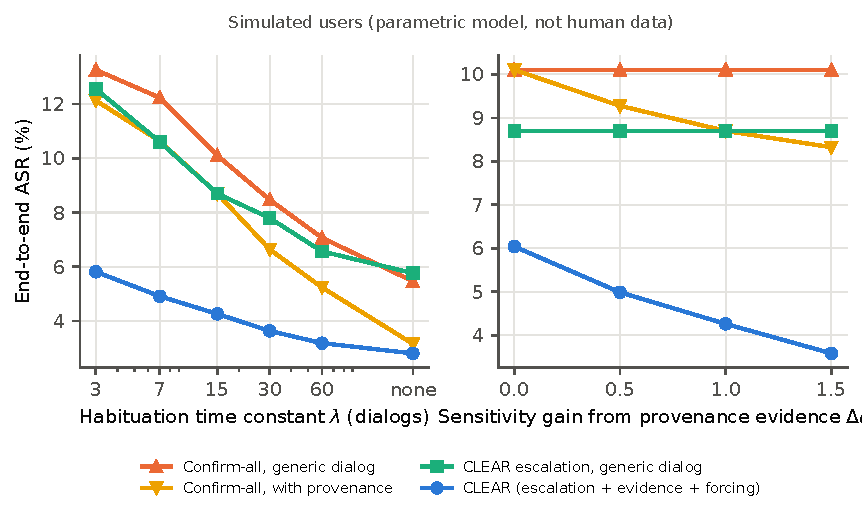
\includegraphics[width=\linewidth]{figures/fig_human_sim.pdf}
\caption{Simulated end-to-end ASR (parametric user model, \emph{not human data}) as a function of the habituation time constant (left) and of the sensitivity gain from provenance evidence (right); other parameters at default.}
\label{fig:human}
\end{figure}

\subsection{Summary of hypotheses}
\begin{table}[h]
\centering\small
\caption{Hypotheses (\cref{sec:intro}; research design in the repository) and outcomes.}
\label{tab:hyp}
\begin{tabular}{p{1.0cm}p{8.6cm}p{4.6cm}}
\toprule
& Hypothesis & Outcome \\
\midrule
H1 & Ideal-user ASR below no defence, allowlist and strict IFC; indistinguishable from confirm-all & \emph{Partly supported}: lower than all three; 0.15\,pp \emph{higher} than confirm-all ($p<10^{-6}$) \\
H2 & Fewer dialogs per benign task than confirm-all & Supported ($-$\dlgReduction\%, $p=\wilcoxP$) \\
H3 & Fail-closed BU above confirm-all-deny; no BU loss with ideal user & Supported (\buClearA{} vs.\ \buCallA\%; \buClearO{} = no defence) \\
H4 & Removing provenance raises ASR; removing $\iota$ costs little; lexical detection fails under evasion & Supported (\cref{tab:ablation}, \cref{fig:curves}) \\
H5 & Lower end-to-end ASR than confirm-all for fallible users & Supported \emph{in simulation only} (\simShare\% of grid) \\
H6 & Provenance raises users' $d'$ without raising workload & \emph{Untested} (user study pending) \\
H7 & Decoding-aware lineage defeats value laundering at no cost on ordinary traffic & Supported for the five value encodings (\laundVtwoVal\% vs.\ \laundVoneMin--\laundVoneMax\%); partly for whole-block encoding: frozen v2 removes about three quarters of the gap; the post-hoc v2.1 closes it (\cref{tab:launder}) \\
H8 & Goal-drift scoring adds security beyond provenance and envelope & \emph{Not supported}: +22\% dialogs on development data, no ASR gain; rejected \\
\bottomrule
\end{tabular}
\end{table}

% =========================================================================
\section{Pre-registered user-study protocol}
\label{sec:study}
The repository contains a complete protocol, consent form, debriefing and
analysis plan. They are ready for ethics review but have not been executed.
\textbf{Design}: a between-subjects $2{\times}2$ factorial crossing
\emph{selectivity} (ask about every side-effecting action vs.\ only about
\clear{} escalations) with \emph{evidence} (generic dialog vs.\ provenance,
excerpt, preview and forcing). The four cells are full \clear{} (A),
confirm-all (B), \clear{} selectivity only (C) and confirm-all with evidence
(D). This design separates the two levers that the simulation predicts to
compound (\cref{fig:human}), and it implements a factorial design recommended
in an earlier iteration of this project. Each participant supervises 16 real GPT-4o trajectories, 4 of which contain a
successful injection. Order is counterbalanced, and attention checks are
embedded. Every escalated action carries the computed consequence preview
(P7). \textbf{Primary outcomes}: prevention of injected actions and completion
of benign tasks, per task. \textbf{Secondary outcomes}: per-dialog
accuracy, SDT $d'$ and $c$, decision time, SUS~\citep{brooke1996sus}, raw
NASA-TLX~\citep{hart1988nasatlx}, and trust in automation~\citep{jian2000trust}.
\textbf{Analysis}: a mixed-effects logistic regression
(\texttt{prevented $\sim$ selective $\times$ evidence + (1|participant) +
(1|scenario)}) testing the two main effects with Holm correction, and
non-inferiority tests for benign completion and workload (A vs.\ B).
\textbf{Power}: each main effect compares 110 against 110 participants. This
detects $d=0.4$ at $\alpha=.05$ with power .80 (100 needed per level). We plan
55 per cell ($N=220$). The interaction is exploratory.
The apparatus logs every decision, response time, forcing answer, envelope edit
and undo. It was verified with an automated browser run of all 16 scenarios in
each of the five conditions: \clear{} and its generic variant raised 13
dialogs, and both confirm-all variants raised 18, with no client errors.

% =========================================================================
\section{Lessons from three design iterations}
\label{sec:lessons}
\clear{} is the third iteration of this project. Its predecessors were built
with different AI research assistants, and their artefacts are preserved in the
repository. Auditing them yielded both design ideas and a methodological
warning.

\paragraph{What was adopted.} The first iteration (\emph{Trust Boundary Lab})
framed the task as \emph{source-to-action review}. That framing became P2's
excerpt display. It also proposed the factorial study design adopted in
\cref{sec:study}. The second iteration (\emph{PROV-Guard}) proposed
decoded-payload provenance, goal-drift scoring and counterfactual previews. Its
decoding idea became decoding-aware lineage (P2, \cref{prop:launder}, E1), and
its preview idea became P7 with \emph{computed} state differences. Goal drift
was tested and rejected (H8).

\paragraph{What was not adopted, and why.} PROV-Guard reported a 92.6\% attack
success rate for binary confirmation dialogs, $d'=4.21$ and a 22.9\% NASA-TLX
reduction for its framework, and $p$-values down to $10^{-16}$ with Cohen's
$d\approx-49$. All of these came from a simulated user whose response to each
interface feature was written into the code. For example, hiding provenance
multiplied the ``cue clarity'' of an attack by 0.42. Re-running its own
pipeline with only these per-feature multipliers set to neutral moves the
ablation results substantially:

\begin{center}\small
\begin{tabular}{lcc}
\toprule
Condition (simulated ASR, \%) & as published & multipliers neutral \\
\midrule
full framework & \auditFullRep & \auditFullNeu \\
without goal drift & \auditNoCgasdRep & \auditNoCgasdNeu \\
without counterfactual preview & \auditNoIcspRep & \auditNoIcspNeu \\
without provenance & \auditNoDlpaRep & \auditNoDlpaNeu \\
binary modal & \auditModalRep & \auditModalNeu \\
\bottomrule
\end{tabular}
\end{center}

The component ranking is therefore an artefact of chosen constants. In that
iteration, the ``Spotlighting'' baseline was a table of catch probabilities,
and no defence had 100\% ASR by construction. Its benchmark is also separable
by a single provenance rule (\cref{sec:v2method}). The first iteration had
briefly scored risk with the ground-truth attack label before correcting
itself.

\paragraph{Reporting rules.} We derive four rules, which this paper follows.
\begin{enumerate}[leftmargin=*,itemsep=1pt]
\item Agent behaviour must come from recorded or live agents, and outcomes from
  the benchmark's own predicates.
\item Simulated humans may generate hypotheses but never results. Every
  parameter is swept and every figure is labelled.
\item Inferential statistics over simulated participants are not reported.
\item Defences are evaluated blind to labels, and synthetic benchmarks are
  checked for trivial separability before use.
\end{enumerate}
As AI assistants increasingly draft research artefacts, we believe such audits
should become routine in HCI-security work.

% =========================================================================
\section{Discussion}
\label{sec:discussion}

\paragraph{Provenance is the robust signal; text signals are cheap but brittle.}
On known templates, instruction-likeness separates attacks almost perfectly.
A mediator built on it would look excellent on static benchmarks: fewer
dialogs, and a detector with near-zero ASR. The same mediator offers no
guarantee once attackers rephrase. AgentDojo's own misspelled
\texttt{ignore\_previous} payload already defeats the lexical detector.
Argument-level provenance is not something the attacker can rephrase away: a
value that only appears in their e-mail is external, whatever the e-mail says.
We recommend that agent platforms make provenance a first-class property of
tool arguments and expose it to users.

\paragraph{The human is a scarce resource; spend attention where it buys security.}
More than half of confirm-all's dialogs (0.41 of 0.79 per benign task) concern
actions that \clear{} does not escalate. Across all held-out episodes they
prevent 23 additional attacks (0.15 percentage points). Their price is
habituation, which the warning literature shows is fast and generalising. \clear{}'s tiering concentrates the strongest
interaction on a small, attack-enriched set. Our simulation suggests that this
selectivity matters as much as better evidence, and that both compound.

\paragraph{Escalations should be verifiable, not persuasive.}
Explanations of an AI's judgement can increase overreliance~\citep{bansal2021whole}.
\clear{}'s dialogs instead state checkable facts---``this account number appears
only in the transaction list''---which lower the cost of
verification~\citep{vasconcelos2023explanations}. The forcing question turns
the most important fact into an action the user must take.

\paragraph{Design implications.}
(1) Treat argument provenance as part of the tool-call API. (2) Budget
interruptions and report dialogs per task alongside ASR. (3) Never execute
irreversible actions silently above the lowest risk tier. (4) Differentiate the
rare high-risk interaction visually \emph{and} behaviourally. (5) Let users
edit the task scope before execution, and keep the compiler out of reach of
injected text. (6) Fail closed when no human is present, and accept that
utility then drops for tasks that genuinely need judgement.

% =========================================================================
\section{Limitations and threats to validity}
\label{sec:validity}

\paragraph{No human-subject data.} All human-factors claims rest on a parametric
model whose parameters are not estimated from people. The model encodes
assumptions drawn from the literature (habituation, forcing, SDT), and our
conclusions are conditional on them. The pre-registered study is the necessary
next step.

\paragraph{Replay instead of live agents.} Replaying recorded trajectories
cannot observe how an agent adapts after a denied call; it might retry or find
another route. A retried attack with the same external target would meet the
same escalation floor, but routes through trusted or user-endorsed values would
not. Conservative utility scoring treats any stopped benign call as task
failure. Replay fidelity is high overall but lower for two pipelines.
Excluding Claude-3-Opus and Llama-3-70B leaves the conclusions unchanged
(repository: \texttt{sensitivity\_high\_fidelity.csv}).

\paragraph{Benchmark scope.} AgentDojo covers four domains and template attacks.
Our detector-evading attacker is a worst case for text signals, but it is not
an optimised attack on provenance. Such an attack would need to make
attacker-chosen values appear in user or trusted sources, or rely on
trusted-derived targets. Output-only manipulation is out of scope by
construction.

\paragraph{Design choices.} The manifest and lexicon were authored by us. Five
changes were made on development data, all disclosed. Held-out evaluation
mitigates but does not eliminate designer bias. Lexical attribution can miss
transformed values. These fall into the weakly tainted ``unattributed'' class
rather than being trusted.

\paragraph{Stress benchmarks and post-hoc fixes.} E2 relies on synthetic,
single-step scenarios that are separable by construction. It can show coverage
and false-escalation behaviour on unfamiliar tools and domains, but not
agent-level security. E1 assumes that agents follow encoded injections as
readily as plain ones. The v2.1 decoder fix was found on held-out data and is
therefore reported separately from the frozen v2. The lexical envelope compiler
can be misled by word forms (``shared''); an LLM-based compiler that sees only
the user's prompt is a natural replacement, but it must itself be shown to be
injection-proof.

\paragraph{Labels.} Call-level labels combine two criteria with high agreement
($\kappa=\labelKappa$). Episode-level outcomes use AgentDojo's predicates and do
not depend on our labels, except in the ideal-user mode.

% =========================================================================
\section{Conclusion and future work}
Prompt-injection defences eventually ask a human. \clear{} makes that question
rare, specific and verifiable. On \nEpisodes{} real agent trajectories it
brings attack success from \asrNone\% to below 1\% while asking half as often as
confirm-all, and it keeps that protection against attackers who evade
text-based detection. Future work will run the pre-registered study, evaluate
live agents with retry behaviour and optimised attacks on provenance, learn
envelope compilers that remain injection-proof, and extend lineage to
multi-agent and computer-use settings.

\section*{Data and code availability}
All source code, configurations, the tool manifest, derived per-episode and
per-call datasets, analysis scripts, figures, tests, the interactive console
and the study materials are available in the project repository
(\url{https://github.com/mazharulmd/HCI}). The raw trajectories are fetched from
the AgentDojo repository (MIT licence) at the pinned commit. The artefacts of
the two earlier iterations are preserved on separate branches, and the audit
in \cref{sec:lessons} can be reproduced from \texttt{results/audit/}.

\section*{Ethics statement}
No human participants were involved. The proposed user study requires approval
by an institutional ethics board before any data collection.

\section*{Declaration of generative AI use}
This project was carried out in three iterations with three AI research
assistants: OpenAI ChatGPT, Google Gemini and Anthropic Claude, operating under
the authors' direction. The final version, including the literature search,
implementation, experiments, audit of the earlier iterations and drafting of
this manuscript, was produced with substantial assistance from Anthropic
Claude. Findings from the earlier iterations that rested on simulated
participants are \emph{not} reported as results (\cref{sec:lessons}). The
authors are responsible for verifying all content. Every numerical result is
generated by the released code, and every reference was checked against a
bibliographic record (verification log in the repository).

\bibliographystyle{plainnat}
\bibliography{references}

\appendix
\section{Per-model results}
\begin{figure}[h]
\centering
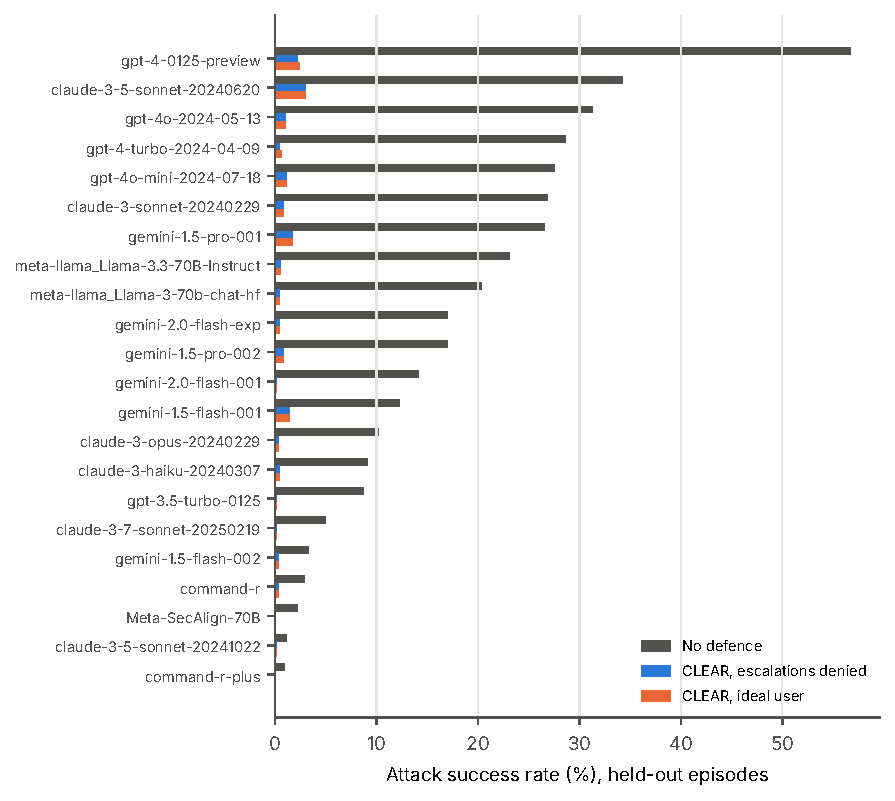
\includegraphics[width=0.72\linewidth]{figures/fig_per_model.pdf}
\caption{ASR per model on held-out episodes.}
\label{fig:permodel}
\end{figure}
\begin{table}[h]
\centering\footnotesize
\caption{Per-model held-out results (ASR and BU in \%; dialogs per benign task).}
\resizebox{\linewidth}{!}{\begin{tabular}{lrrrrrr}
\toprule
Model & $n$ & ASR none & ASR CLEAR & BU none & Dialogs CLEAR & Dialogs confirm-all \\
\midrule
gpt-4-0125-preview & 629 & 56.8 & 2.4 & 66.0 & 0.44 & 0.92 \\
claude-3-5-sonnet-20240620 & 625 & 34.2 & 3.0 & 80.2 & 0.48 & 0.94 \\
gpt-4o-2024-05-13 & 380 & 31.3 & 1.1 & 63.3 & 0.22 & 0.43 \\
gpt-4-turbo-2024-04-09 & 629 & 28.6 & 0.6 & 64.9 & 0.39 & 0.84 \\
gpt-4o-mini-2024-07-18 & 629 & 27.5 & 1.1 & 69.1 & 0.59 & 1.15 \\
claude-3-sonnet-20240229 & 629 & 26.9 & 0.8 & 53.6 & 0.39 & 0.68 \\
gemini-1.5-pro-001 & 629 & 26.6 & 1.7 & 45.4 & 0.29 & 0.61 \\
Llama-3.3-70B-Instruct & 949 & 23.1 & 0.5 & 57.7 & 0.43 & 0.95 \\
Llama-3-70b-chat-hf & 629 & 20.3 & 0.5 & 33.0 & 0.21 & 0.59 \\
gemini-2.0-flash-exp & 629 & 17.0 & 0.5 & 46.4 & 0.25 & 0.59 \\
gemini-1.5-pro-002 & 629 & 17.0 & 0.8 & 60.8 & 0.36 & 0.81 \\
gemini-2.0-flash-001 & 949 & 14.1 & 0.1 & 43.3 & 0.33 & 0.62 \\
gemini-1.5-flash-001 & 629 & 12.2 & 1.4 & 39.2 & 0.32 & 0.63 \\
claude-3-opus-20240229 & 629 & 10.2 & 0.3 & 69.1 & 0.45 & 0.81 \\
claude-3-haiku-20240307 & 629 & 9.1 & 0.5 & 39.2 & 0.39 & 0.70 \\
gpt-3.5-turbo-0125 & 629 & 8.7 & 0.2 & 35.1 & 0.61 & 1.11 \\
claude-3-7-sonnet-20250219 & 949 & 5.0 & 0.1 & 88.7 & 0.52 & 0.99 \\
gemini-1.5-flash-002 & 629 & 3.3 & 0.3 & 38.1 & 0.19 & 0.51 \\
command-r & 629 & 2.9 & 0.3 & 25.8 & 0.36 & 0.97 \\
Meta-SecAlign-70B & 949 & 2.2 & 0.0 & 77.3 & 0.59 & 1.12 \\
claude-3-5-sonnet-20241022 & 629 & 1.1 & 0.2 & 80.4 & 0.43 & 0.90 \\
command-r-plus & 629 & 1.0 & 0.0 & 23.7 & 0.16 & 0.43 \\
\bottomrule
\end{tabular}
}
\end{table}

\section{Call-level ROC}
\begin{figure}[h]
\centering
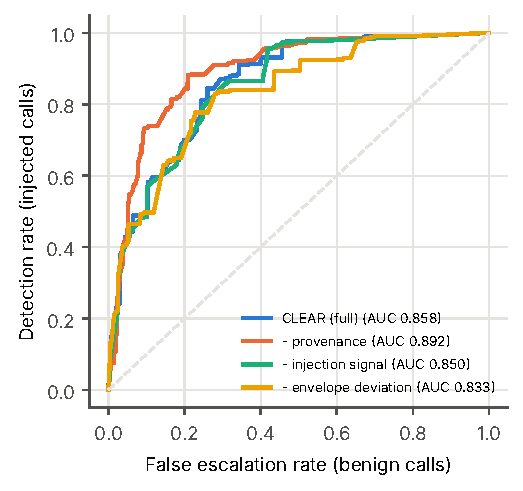
\includegraphics[width=0.5\linewidth]{figures/fig_roc.pdf}
\caption{ROC of the risk score for injected versus benign side-effecting calls (held-out, template attack).}
\end{figure}

\end{document}
